\section{Tests and Results}
\label{sec:testsResults}
\subsection{Metrics}
\par The corresponding results for each experimental configuration were registered in the following formats:
		\begin{itemize}
			\item{} confusion matrices.
			\item{} values of accuracy and their respective standard deviations.
			\item{} EER curves.
		\end{itemize}
\par In the confusion matrix example, shown as being the Table \ref{tab:confusionMatrixSample}, the \textbf{lines} represent the \textbf{predicted classes} and the \textbf{columns} the \textbf{actual classes}, where:
\begin{itemize}
			\item{}\textbf{TP} is the number of true items classified as such, i.e., the \textit{True Positives}.
			\item{}\textbf{TN} is the number of false items classified as such, i.e., the \textit{True Negatives}.
			\item{}\textbf{FN} is the number of of true items classified as false, i.e., \textit{False Negatives}.
			\item{}\textbf{FP} is the number of false items classified as true, i.e., \textit{False Positives}.
		\end{itemize}
\begin{table}
\newcommand{\mc}[3]{\multicolumn{#1}{#2}{#3}}
\definecolor{tcB}{rgb}{0.447059,0.74902,0.266667}
\definecolor{tcC}{rgb}{0,0,0}
\definecolor{tcD}{rgb}{0,0.4,0.701961}
\definecolor{tcA}{rgb}{0.65098,0.65098,0.65098}
\begin{center}
	\begin{tabular}{ccc}
		% use packages: color,colortbl
		\mc{1}{l}{} & \mc{1}{>{\columncolor{tcA}}c}{\textbf{Verdadeiro}} & \mc{1}{>{\columncolor{tcA}}c}{\textbf{Falso}}\\

		\mc{1}{>{\columncolor{tcA}}r}{\textbf{Verdadeiro}} & \mc{1}{>{\columncolor{tcB}}c}{\textcolor{tcC}{VV}} & \mc{1}{>{\columncolor{tcD}}c}{\textcolor{tcC}{FV}}\\

		\mc{1}{>{\columncolor{tcA}}r}{\textbf{Falso}} & \mc{1}{>{\columncolor{tcD}}c}{\textcolor{tcC}{FF}} & \mc{1}{>{\columncolor{tcB}}c}{\textcolor{tcC}{VF}}
	\end{tabular}
	\caption{Exemplo de matriz de confusão}
	\label{tab:confusionMatrixSample}
\end{center}
\end{table}

To be calculated, the value of accuracy in a classification task is based on \textit{TP}, \textit{TN}, and the number of elements (\textit{N}), as shown in Equation \ref{eq:calculoDaAcuracia}.
\begin{equation}
\text{value of accuracy} = \dfrac{TP + TN}{N} \qquad.
\label{eq:calculoDaAcuracia}
\end{equation}
\par In order to calculate the EER, the values of \textit{FP} and \textit{FN} are taken into account \cite{ghazali2018recent}. From them, the \textit{False Acceptance Rate (\textbf{FAR})}, as shown in the Equation \ref{eq:FAR}, and \textit{False Rejection Rate (\textbf{FRR})}, as shown in Equation \ref{eq:FRR}, are obtained.
\begin{equation}
\text{FAR}=\dfrac{FP}{TN+FP} \qquad.
\label{eq:FAR}
\end{equation}
\begin{equation}
\text{FRR}=\dfrac{FN}{TP+FN} \qquad.
\label{eq:FRR}
\end{equation}
\par Confusion matrices are calculated for a sufficient number of times until \textbf{\textit{FAR} is equal to, or close to, \textit{FRR}}. At each cycle, the feature vectors are switched randomly so that different values are obtained. For some cases, over 12000 iterations were required in order to find the configuration that made \textit{FAR=FRR}.
\\
\par At each iteration, the values of FAR and FRR are stored in two vectors, being one for each parameter, so that the vector belonging to FAR is sorted in ascending order and the other in decreasing order. These points are depicted on the EER curve, together with a diagonal straight line, creating a \textit{Detection Error Trade off (DET)} plot. The effective value of ERR matches the intersection of the diagonal line with the curve defined by FAR and FRR.
\subsection{Experiments}
	\par Figure \ref{fig:paraconsistentfull} combines the results obtained with various wavelet filters and the auditory Bark and Mel scales. Since the bars lengths in blue represent the logarithmic distances from $P=(G_1,G_2)$ to the corner $(1,0)$ of the paraconsistent plane, according to the wavelet filter and the auditory scale used, we can state that the leftest the horizontal bars go, the better the separability between the classes. As can be seen from those combinations, \textbf{Haar wavelets + Bark scale} provide the shortest distance. To complement the information reported graphically, Tables \ref{tab:distParacomFrom10Bark_1}, \ref{tab:distParacomFrom10Bark_2}, \ref{tab:distParacomFrom10Mel_1}, and \ref{tab:distParacomFrom10Mel_2} contain the specific values displayed in that Figure.
	\\
	\begin{figure}[H]
		\centering
		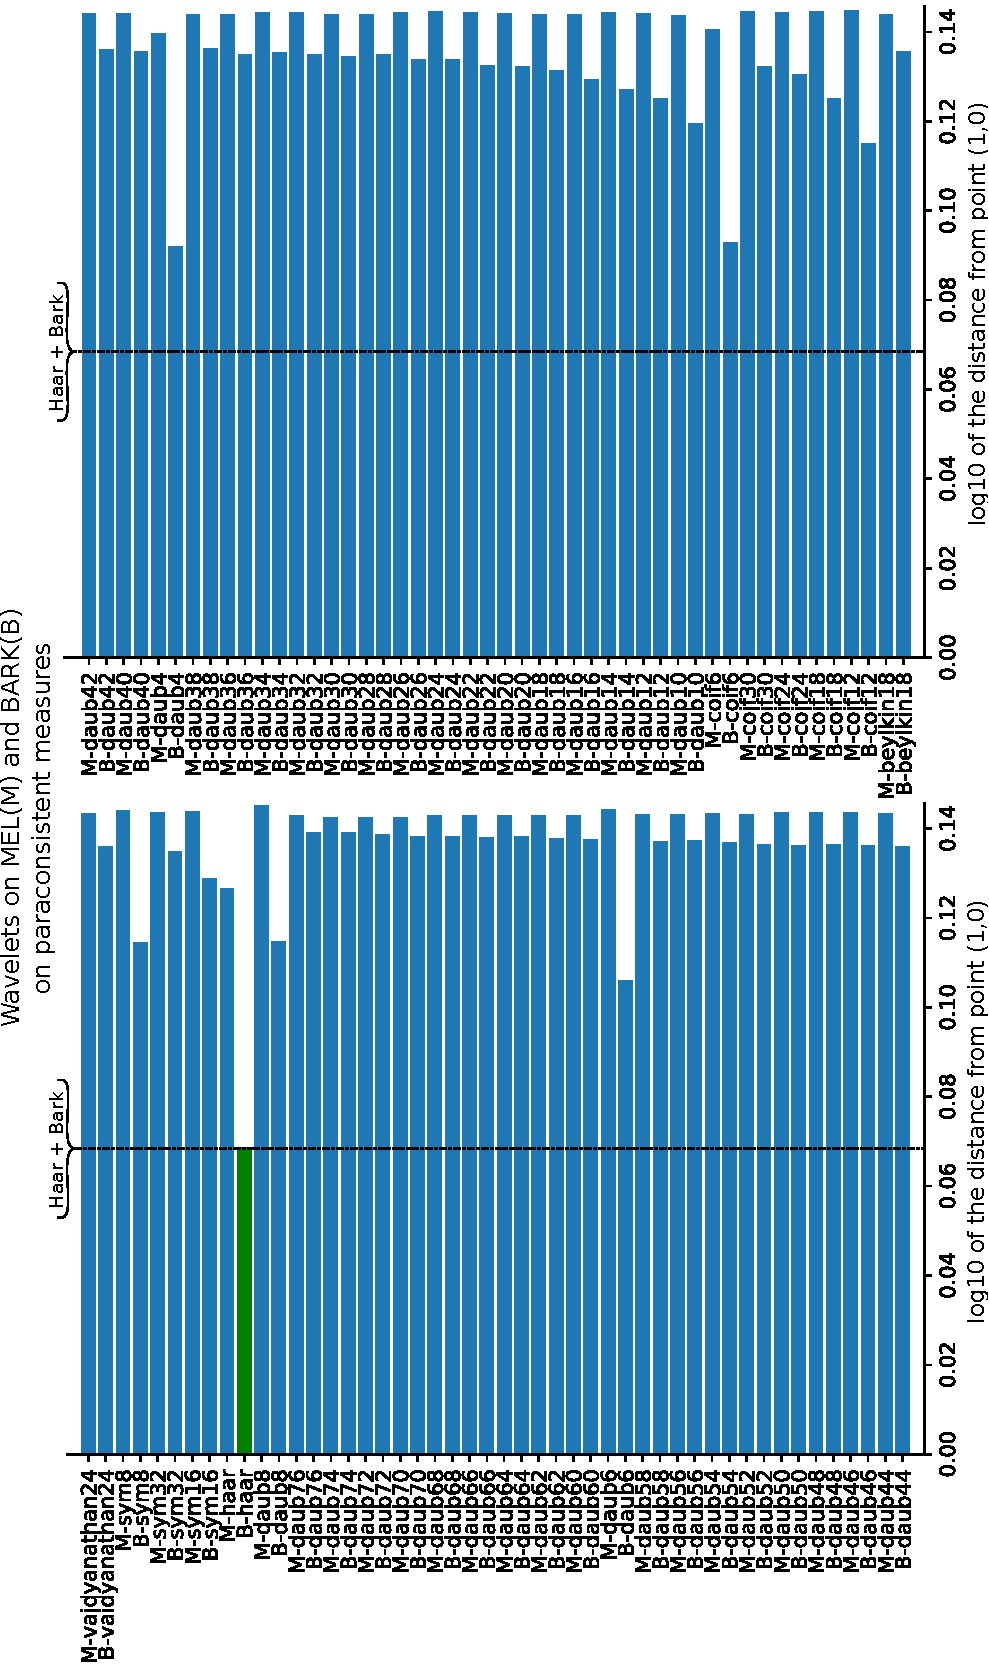
\includegraphics[angle=-90,scale=.49]{images/results/paraconsistentPlane/ParaconsistentFull.pdf}
		\caption{Distances from $P=(G_1,G_2)$ to the corner $(1,0)$ in the paraconsistent plane.}
		\label{fig:paraconsistentfull}
	\end{figure}
	\par Overall, the \textbf{wavelet + Bark} combination consistently presented \textbf{better} results in comparison with the respective \textbf{wavelet + Mel} combinations. Based on the behavior of the best and worst wavelets, a natural question is why \textbf{Haar} filters have provided the best results. Particularly interesting is the fact that \textbf{Haar} and \textbf{Daubechies 18} \textit{wavelet} filters provided, respectively, the best and worst results associated with the Bark scale. In contrast, adopting the \textit{Mel} scale, \textbf{Daubechies 58} was the best filter and \textbf{Coiflets 18} the worst.
	\\
	\par In regard to the filter's phase and frequency responses, we know that Haar presents a frequency response curve that is mostly far from the ideal, as it is just a first-order finite impulse response (FIR) filter \cite{WaveletPropertiesBrowser}. Therefore, specific frequency sub-bands are undoubtedly contaminated with spectral content from adjacent sub-bands. Additionally, Haar is the only family of orthogonal \textit{wavelet} filters exhibiting linear phase response. Hence, we can note that a non-rigorous frequency response associated with a linear phase response is the best alternative to solve our problem. Notably, the same behavior has been observed with experiments in different sub-fields of signal processing \cite{guido2}\cite{guido3}\cite{guido4}. 
	\\
	\par From the point of view of the auditory Bark and Mel scales, it is relevant to note that the former, not the latter, presents the best results. Nevertheless, the latter is the one optimized for voice and speech signals. Thus, the \textbf{noisy profile} of the spoofed signals, containing, unlike the genuine voices, notorious random components of high frequencies, was better detected with an auditory scale adequate to handle audio signals in general, not speech and voice. This is another relevant point to address. 
	
	\begin{center}
	\newcommand{\mc}[3]{\multicolumn{#1}{#2}{#3}}
	\definecolor{tcB}{rgb}{0.447059,0.74902,0.266667}
	\definecolor{tcA}{rgb}{0.65098,0.65098,0.65098}
	\definecolor{tcC}{rgb}{0,0.8,1}
	
	\begin{longtable}[h]{|c|c|c|c|c|}
		
		% Columns headers
		\hline
		\mc{1}{|>{\columncolor{tcA}}c|}{Mel/Bark}&\mc{1}{|>{\columncolor{tcA}}c|}{Wavelet}&\mc{1}{|>{\columncolor{tcA}}c|}{G1}&\mc{1}{|>{\columncolor{tcA}}c|}{G2}&\mc{1}{|>{\columncolor{tcA}}c|}{Distância de (1,0)}\\\hline
		\endfirsthead
		
		\mc{3}{c}{{\tablename\ \thetable : Continuação da página anterior}} \\\hline
		% Columns headers
		\mc{1}{|>{\columncolor{tcA}}c|}{Mel/Bark}&\mc{1}{|>{\columncolor{tcA}}c|}{Wavelet}&\mc{1}{|>{\columncolor{tcA}}c|}{G1}&\mc{1}{|>{\columncolor{tcA}}c|}{G2}&\mc{1}{|>{\columncolor{tcA}}c|}{Distance to (1,0)}\\\hline
		\endhead
		
		\hline \mc{2}{c}{{Continua na próxima página}} \\
		\endfoot
		\endlastfoot
		
		% Color of the first line
		\rowcolor{tcB}
		
		% Loads data from tables/results/paraconsistentPlane/distParacomFrom10.csv
		\csvreader[
		no head,
		late after line=\\\hline\rowcolor{tcC},%
		separator=comma,
		filter={\value{csvrow}<4},
		]{../monography/tables/results/paraconsistentPlane/distParacomFrom10.csv}{
			1=\melBark,
			2=\wavelet,
			3=\gOne,
			4=\gTwo,
			5=\distance
		}{
			\melBark&
			\wavelet&
			\StrSubstitute[0]{\gOne}{.}{,}&
			\StrSubstitute[0]{\gTwo}{.}{,}&
			\StrSubstitute[0]{\distance}{.}{,}
		}
		
		\rowcolor{white}
		\caption{As 5 primeiras combinações Wavelet \textit{x} Mel/Bark ordenadas pela distância do vértice (1,0) no plano paraconsistente.}
		\label{tab:distParacomFrom10BarkAndMel}
	\end{longtable}
\end{center}
	
	\par Since the combination \textbf{Haar+Bark} was the best one, we now search for the \textbf{maximum accuracy and minimum EER} that can be achieved. To do so, two classifiers were adopted to receive those features as input: a modest pattern-matching approach, based on Euclidean and Manhattan distances, and a knowledge-based one, based on an SVM. 
	\\
	\par To perform the classifications, we randomly selected $M\%$ of our feature vectors, i.e., $\frac{410 \cdot M}{100} + \frac{410 \cdot M}{100} = 8.2 \cdot M$ to play the role of template models, and the corresponding remaining fraction, i.e., $(100-M)\%$ for testing, where $M=10, 20, 30, 40, 50$. For each value of $M$, 300 random selections were performed. In the distance-based classification strategy, the distance from each feature vector reserved for testing the proposed approach to all the template models was registered and, then, the smallest one was used to label the feature vector being classified. Essentially, this corresponds to the traditional K-Nearest Neighbors (K-NN) classifier with $K=1$.     

		\begin{table}[h]
	\newcommand{\mc}[3]{\multicolumn{#1}{#2}{#3}}
	\definecolor{tcA}{rgb}{0.65098,0.65098,0.65098}
	\definecolor{tcB}{rgb}{0.447059,0.74902,0.266667}
	\begin{center}
		\begin{tabular}{|l|l|l|}\hline
			% use packages: color,colortbl
			\rowcolor{tcA}
			\textbf{Tamanho do modelo} & \textbf{Acurácia mínima} & \textbf{Acurácia máxima}\\\hline
			\rowcolor{tcB}
			\mc{1}{|c|}{10\%} & \mc{1}{c|}{0,6666} & \mc{1}{c|}{0,8861}\\\hline
			\rowcolor{tcB}
			\mc{1}{|c|}{20\%} & \mc{1}{c|}{0,7439} & \mc{1}{c|}{0,8902}\\\hline
			\rowcolor{tcB}
			\mc{1}{|c|}{30\%} & \mc{1}{c|}{0,7665} & \mc{1}{c|}{0,8919}\\\hline
			\rowcolor{tcB}
			\mc{1}{|c|}{40\%} & \mc{1}{c|}{0,7784} & \mc{1}{c|}{0,9024}\\\hline
			\rowcolor{tcB}
			\mc{1}{|c|}{50\%} & \mc{1}{c|}{0,7804} & \mc{1}{c|}{0,9097}\\\hline
		\end{tabular}
	\end{center}
	\caption{Resultados do experimento 02}
	\label{tab:experiment02Results}
\end{table}
		
		\FloatBarrier
		
		\par The corresponding results are shown in Tables \ref{tab:experiment02ResultsEuclidian} and \ref{tab:experiment02ResultsManhattan}. Particularly notable are the EER values, which balance the rates of false positives and false negatives. Specific details for the Euclidean distance classifier are shown in Tables \ref{tab:classifier_Euclidian_10_best}, \ref{tab:classifier_Euclidian_10_worse},
		\ref{tab:classifier_Euclidian_20_best}, \ref{tab:classifier_Euclidian_20_worse}, 
		\ref{tab:classifier_Euclidian_30_best}, \ref{tab:classifier_Euclidian_30_worse}, 
		\ref{tab:classifier_Euclidian_40_best}, \ref{tab:classifier_Euclidian_40_worse}, 
		\ref{tab:classifier_Euclidian_50_best},  and \ref{tab:classifier_Euclidian_50_worse}. The corresponding plots are depicted in Figures \ref{fig:classifiereuclidian10}, \ref{fig:classifiereuclidian20}, \ref{fig:classifiereuclidian30}, \ref{fig:classifiereuclidian40}, and \ref{fig:classifiereuclidian50}. For Manhattan distances,  Tables \ref{tab:classifier_Manhattan_10_best}, \ref{tab:classifier_Manhattan_10_worst}, 
		\ref{tab:classifier_Manhattan_20_best}, \ref{tab:classifier_Manhattan_20_worst}, 
		\ref{tab:classifier_Manhattan_30_best}, \ref{tab:classifier_Manhattan_30_worse}, 
		\ref{tab:classifier_Manhattan_40_best}, \ref{tab:classifier_Manhattan_40_worse}, 
		\ref{tab:classifier_Manhattan_50_best},
		\ref{tab:classifier_Manhattan_50_worse} 
		can be consulted together with the respective plots in Figures \ref{fig:classifiermanhattan10}, \ref{fig:classifiermanhattan20}, \ref{fig:classifiermanhattan30}, \ref{fig:classifiermanhattan40}, and \ref{fig:classifiermanhattan50}.

		\begin{table}[H] 					\newcommand{\mc}[3]{\multicolumn{#1}{#2}{#3}} 					\definecolor{tcB}{rgb}{0.447059,0.74902,0.266667} 					\definecolor{tcC}{rgb}{0,0,0} 					\definecolor{tcD}{rgb}{0,0.5,1} 					\definecolor{tcA}{rgb}{0.65098,0.65098,0.65098} 					\begin{center} 						\subfloat[Melhor matriz de confusão]{ 							\begin{tabular}{ccc} 								\mc{1}{l}{} & \mc{1}{>{\columncolor{tcA}}c}{\textbf{genuíno}} & \mc{1}{>{\columncolor{tcA}}c}{\textbf{falseado}}\\ 								\mc{1}{>{\columncolor{tcA}}r}{\textbf{genuíno}} & \mc{1}{>{\columncolor{tcB}}c}{\textcolor{tcC}{363}} & \mc{1}{>{\columncolor{tcD}}c}{\textcolor{tcC}{14}}\\ 								\mc{1}{>{\columncolor{tcA}}r}{\textbf{falseado}} & \mc{1}{>{\columncolor{tcD}}c}{\textcolor{tcC}{6}} & \mc{1}{>{\columncolor{tcB}}c}{\textcolor{tcC}{355}} 							\end{tabular} 							\label{tab:classifier_Euclidian_10_best} 						} 						\qquad 						\subfloat[Pior matriz de confusão]{ 							\begin{tabular}{ccc} 								\mc{1}{l}{} & \mc{1}{>{\columncolor{tcA}}c}{\textbf{genuíno}} & \mc{1}{>{\columncolor{tcA}}c}{\textbf{falseado}}\\ 								\mc{1}{>{\columncolor{tcA}}r}{\textbf{genuíno}} & \mc{1}{>{\columncolor{tcB}}c}{\textcolor{tcC}{275}} & \mc{1}{>{\columncolor{tcD}}c}{\textcolor{tcC}{10}}\\ 								\mc{1}{>{\columncolor{tcA}}r}{\textbf{falseado}} & \mc{1}{>{\columncolor{tcD}}c}{\textcolor{tcC}{94}} & \mc{1}{>{\columncolor{tcB}}c}{\textcolor{tcC}{359}} 							\end{tabular} 							\label{tab:classifier_Euclidian_10_worse} 						} 					\end{center} 					\caption{Matrizes de confusão para distância Euclidiana com modelo a 10\%} 				\end{table}
		\begin{table}[h]
\newcommand{\mc}[3]{\multicolumn{#1}{#2}{#3}}
\definecolor{tcB}{rgb}{0.447059,0.74902,0.266667}
\definecolor{tcC}{rgb}{0,0,0}
\definecolor{tcD}{rgb}{0,0.4,0.701961}
\definecolor{tcA}{rgb}{0.65098,0.65098,0.65098}
\begin{center}
	\begin{tabular}{ccc}
		% use packages: color,colortbl
		\mc{1}{l}{} & \mc{1}{>{\columncolor{tcA}}c}{\textbf{genuíno}} & \mc{1}{>{\columncolor{tcA}}c}{\textbf{regravado}}\\

		\mc{1}{>{\columncolor{tcA}}r}{\textbf{genuíno}} & \mc{1}{>{\columncolor{tcB}}c}{\textcolor{tcC}{308}} & \mc{1}{>{\columncolor{tcD}}c}{\textcolor{tcC}{50}}\\

		\mc{1}{>{\columncolor{tcA}}r}{\textbf{regravado}} & \mc{1}{>{\columncolor{tcD}}c}{\textcolor{tcC}{20}} & \mc{1}{>{\columncolor{tcB}}c}{\textcolor{tcC}{278}}
	\end{tabular}
	\caption{Melhor matriz de confusão para o classificador por distâncias Euclidianas com o uso de 20\% da base para modelagem}
	\label{tab:classifier_Euclidian_20_best}
\end{center}
\end{table}

\begin{table}[h]
	\newcommand{\mc}[3]{\multicolumn{#1}{#2}{#3}}
	\definecolor{tcB}{rgb}{0.447059,0.74902,0.266667}
	\definecolor{tcC}{rgb}{0,0,0}
	\definecolor{tcD}{rgb}{0,0.4,0.701961}
	\definecolor{tcA}{rgb}{0.65098,0.65098,0.65098}
	\begin{center}
		\begin{tabular}{ccc}
			% use packages: color,colortbl
			\mc{1}{l}{} & \mc{1}{>{\columncolor{tcA}}c}{\textbf{genuíno}} & \mc{1}{>{\columncolor{tcA}}c}{\textbf{regravado}}\\
			
			\mc{1}{>{\columncolor{tcA}}r}{\textbf{genuíno}} & \mc{1}{>{\columncolor{tcB}}c}{\textcolor{tcC}{295}} & \mc{1}{>{\columncolor{tcD}}c}{\textcolor{tcC}{137}}\\
			
			\mc{1}{>{\columncolor{tcA}}r}{\textbf{regravado}} & \mc{1}{>{\columncolor{tcD}}c}{\textcolor{tcC}{33}} & \mc{1}{>{\columncolor{tcB}}c}{\textcolor{tcC}{191}}
		\end{tabular}
		\caption{Pior matriz de confusão para o classificador por distâncias Euclidianas com o uso de 20\% da base para modelagem}
		\label{tab:classifier_Euclidian_20_worse}
	\end{center}
\end{table}

		\begin{table}[H] 					\newcommand{\mc}[3]{\multicolumn{#1}{#2}{#3}} 					\definecolor{tcB}{rgb}{0.447059,0.74902,0.266667} 					\definecolor{tcC}{rgb}{0,0,0} 					\definecolor{tcD}{rgb}{0,0.5,1} 					\definecolor{tcA}{rgb}{0.65098,0.65098,0.65098} 					\begin{center} 		\caption{Matrizes de confusão para distância Euclidiana com modelo a 30\%}				\subfloat[Melhor matriz de confusão]{ 							\begin{tabular}{ccc} 								\mc{1}{l}{} & \mc{1}{>{\columncolor{tcA}}c}{\textbf{genuíno}} & \mc{1}{>{\columncolor{tcA}}c}{\textbf{falseado}}\\ 								\mc{1}{>{\columncolor{tcA}}r}{\textbf{genuíno}} & \mc{1}{>{\columncolor{tcB}}c}{\textcolor{tcC}{283}} & \mc{1}{>{\columncolor{tcD}}c}{\textcolor{tcC}{8}}\\ 								\mc{1}{>{\columncolor{tcA}}r}{\textbf{falseado}} & \mc{1}{>{\columncolor{tcD}}c}{\textcolor{tcC}{4}} & \mc{1}{>{\columncolor{tcB}}c}{\textcolor{tcC}{279}} 							\end{tabular} 							\label{tab:classifier_Euclidian_30_best} 						} 						\qquad 						\subfloat[Pior matriz de confusão]{ 							\begin{tabular}{ccc} 								\mc{1}{l}{} & \mc{1}{>{\columncolor{tcA}}c}{\textbf{genuíno}} & \mc{1}{>{\columncolor{tcA}}c}{\textbf{falseado}}\\ 								\mc{1}{>{\columncolor{tcA}}r}{\textbf{genuíno}} & \mc{1}{>{\columncolor{tcB}}c}{\textcolor{tcC}{258}} & \mc{1}{>{\columncolor{tcD}}c}{\textcolor{tcC}{20}}\\ 								\mc{1}{>{\columncolor{tcA}}r}{\textbf{falseado}} & \mc{1}{>{\columncolor{tcD}}c}{\textcolor{tcC}{29}} & \mc{1}{>{\columncolor{tcB}}c}{\textcolor{tcC}{267}} 							\end{tabular} 							\label{tab:classifier_Euclidian_30_worse} 						} 					\\Fonte: Elaborado pelo autor, 2021.		\end{center} 					 				\end{table}
		\begin{table}[h]
\newcommand{\mc}[3]{\multicolumn{#1}{#2}{#3}}
\definecolor{tcB}{rgb}{0.447059,0.74902,0.266667}
\definecolor{tcC}{rgb}{0,0,0}
\definecolor{tcD}{rgb}{0,0.4,0.701961}
\definecolor{tcA}{rgb}{0.65098,0.65098,0.65098}
\begin{center}
	\begin{tabular}{ccc}
		% use packages: color,colortbl
		\mc{1}{l}{} & \mc{1}{>{\columncolor{tcA}}c}{\textbf{Verdadeiro}} & \mc{1}{>{\columncolor{tcA}}c}{\textbf{Falso}}\\

		\mc{1}{>{\columncolor{tcA}}r}{\textbf{Verdadeiro}} & \mc{1}{>{\columncolor{tcB}}c}{\textcolor{tcC}{233}} & \mc{1}{>{\columncolor{tcD}}c}{\textcolor{tcC}{35}}\\

		\mc{1}{>{\columncolor{tcA}}r}{\textbf{Falso}} & \mc{1}{>{\columncolor{tcD}}c}{\textcolor{tcC}{13}} & \mc{1}{>{\columncolor{tcB}}c}{\textcolor{tcC}{211}}
	\end{tabular}
	\caption{Tabela de confusão para classificador Euclidiano 40\%}
	\label{tab:classifier_Euclidian_40}
\end{center}
\end{table}

		\begin{table}[H]
	\newcommand{\mc}[3]{\multicolumn{#1}{#2}{#3}}
	\definecolor{tcB}{rgb}{0.447059,0.74902,0.266667}
	\definecolor{tcC}{rgb}{0,0,0}
	\definecolor{tcD}{rgb}{0,0.5,1}
	\definecolor{tcA}{rgb}{0.65098,0.65098,0.65098}
	\begin{center}
		\subfloat[Best matrix]{
			\begin{tabular}{ccc}
				% use packages: color,colortbl
				\mc{1}{l}{} & \mc{1}{>{\columncolor{tcA}}c}{\textbf{genuine}} & \mc{1}{>{\columncolor{tcA}}c}{\textbf{spoofed}}\\
				
				\mc{1}{>{\columncolor{tcA}}r}{\textbf{genuine}} & \mc{1}{>{\columncolor{tcB}}c}{\textcolor{tcC}{195}} & \mc{1}{>{\columncolor{tcD}}c}{\textcolor{tcC}{29}}\\
				
				\mc{1}{>{\columncolor{tcA}}r}{\textbf{spoofed}} & \mc{1}{>{\columncolor{tcD}}c}{\textcolor{tcC}{10}} & \mc{1}{>{\columncolor{tcB}}c}{\textcolor{tcC}{176}}
			\end{tabular}
			\label{tab:classifier_Euclidian_50_best}
		}
		\qquad
		\subfloat[Worst matrix]{
			\begin{tabular}{ccc}
				% use packages: color,colortbl
				\mc{1}{l}{} & \mc{1}{>{\columncolor{tcA}}c}{\textbf{genuine}} & \mc{1}{>{\columncolor{tcA}}c}{\textbf{spoofed}}\\
				
				\mc{1}{>{\columncolor{tcA}}r}{\textbf{genuine}} & \mc{1}{>{\columncolor{tcB}}c}{\textcolor{tcC}{193}} & \mc{1}{>{\columncolor{tcD}}c}{\textcolor{tcC}{79}}\\
				
				\mc{1}{>{\columncolor{tcA}}r}{\textbf{spoofed}} & \mc{1}{>{\columncolor{tcD}}c}{\textcolor{tcC}{12}} & \mc{1}{>{\columncolor{tcB}}c}{\textcolor{tcC}{126}}
			\end{tabular}
			\label{tab:classifier_Euclidian_50_worse}
		}
	\end{center}
	\caption{Confusion matrices for Euclidian distance classifier at 50\% model}
\end{table}
		\begin{table}[h] 					\newcommand{\mc}[3]{\multicolumn{#1}{#2}{#3}} 					\definecolor{tcB}{rgb}{0.447059,0.74902,0.266667} 					\definecolor{tcC}{rgb}{0,0,0} 					\definecolor{tcD}{rgb}{0,0.5,1} 					\definecolor{tcA}{rgb}{0.65098,0.65098,0.65098} 					\begin{center} 						\subfloat[Melhor matriz de confusão]{ 							\begin{tabular}{ccc} 								\mc{1}{l}{} & \mc{1}{>{\columncolor{tcA}}c}{\textbf{genuíno}} & \mc{1}{>{\columncolor{tcA}}c}{\textbf{falsificado}}\\ 								\mc{1}{>{\columncolor{tcA}}r}{\textbf{genuíno}} & \mc{1}{>{\columncolor{tcB}}c}{\textcolor{tcC}{365}} & \mc{1}{>{\columncolor{tcD}}c}{\textcolor{tcC}{14}}\\ 								\mc{1}{>{\columncolor{tcA}}r}{\textbf{falsificado}} & \mc{1}{>{\columncolor{tcD}}c}{\textcolor{tcC}{4}} & \mc{1}{>{\columncolor{tcB}}c}{\textcolor{tcC}{355}} 							\end{tabular} 							\label{tab:classifier_Manhattan_10_best} 						} 						\qquad 						\subfloat[Pior matriz de confusão]{ 							\begin{tabular}{ccc} 								\mc{1}{l}{} & \mc{1}{>{\columncolor{tcA}}c}{\textbf{genuíno}} & \mc{1}{>{\columncolor{tcA}}c}{\textbf{falsificado}}\\ 								\mc{1}{>{\columncolor{tcA}}r}{\textbf{genuíno}} & \mc{1}{>{\columncolor{tcB}}c}{\textcolor{tcC}{289}} & \mc{1}{>{\columncolor{tcD}}c}{\textcolor{tcC}{11}}\\ 								\mc{1}{>{\columncolor{tcA}}r}{\textbf{falsificado}} & \mc{1}{>{\columncolor{tcD}}c}{\textcolor{tcC}{80}} & \mc{1}{>{\columncolor{tcB}}c}{\textcolor{tcC}{358}} 							\end{tabular} 							\label{tab:classifier_Manhattan_10_worse} 						} 					\end{center} 					\caption{Matrizes de confusão para distância Manhattan com modelo a 10\%} 				\end{table}
		\begin{table}[h]
	\newcommand{\mc}[3]{\multicolumn{#1}{#2}{#3}}
	\definecolor{tcB}{rgb}{0.447059,0.74902,0.266667}
	\definecolor{tcC}{rgb}{0,0,0}
	\definecolor{tcD}{rgb}{0,0.5,1}
	\definecolor{tcA}{rgb}{0.65098,0.65098,0.65098}
	\begin{center}
		\subfloat[Melhor matriz]{
			\begin{tabular}{ccc}
				% use packages: color,colortbl
				\mc{1}{l}{} & \mc{1}{>{\columncolor{tcA}}c}{\textbf{Verdadeiro}} & \mc{1}{>{\columncolor{tcA}}c}{\textbf{Falso}}\\
				
				\mc{1}{>{\columncolor{tcA}}r}{\textbf{Verdadeiro}} & \mc{1}{>{\columncolor{tcB}}c}{\textcolor{tcC}{308}} & \mc{1}{>{\columncolor{tcD}}c}{\textcolor{tcC}{44}}\\
				
				\mc{1}{>{\columncolor{tcA}}r}{\textbf{Falso}} & \mc{1}{>{\columncolor{tcD}}c}{\textcolor{tcC}{20}} & \mc{1}{>{\columncolor{tcB}}c}{\textcolor{tcC}{284}}
			\end{tabular}
			\label{tab:classifier_Manhattan_20_best}
		}
		\qquad
		\subfloat[Pior matriz]{
			\begin{tabular}{ccc}
				% use packages: color,colortbl
				\mc{1}{l}{} & \mc{1}{>{\columncolor{tcA}}c}{\textbf{Verdadeiro}} & \mc{1}{>{\columncolor{tcA}}c}{\textbf{Falso}}\\
				
				\mc{1}{>{\columncolor{tcA}}r}{\textbf{Verdadeiro}} & \mc{1}{>{\columncolor{tcB}}c}{\textcolor{tcC}{316}} & \mc{1}{>{\columncolor{tcD}}c}{\textcolor{tcC}{149}}\\
				
				\mc{1}{>{\columncolor{tcA}}r}{\textbf{Falso}} & \mc{1}{>{\columncolor{tcD}}c}{\textcolor{tcC}{12}} & \mc{1}{>{\columncolor{tcB}}c}{\textcolor{tcC}{179}}
			\end{tabular}
			\label{tab:classifier_Manhattan_20_worst}
		}
	\end{center}
	\caption{Matrizes de confusão para o classificador por distâncias Manhattan com o uso de 20\% da base para modelagem}
\end{table}

		\begin{table}[h] 					\newcommand{\mc}[3]{\multicolumn{#1}{#2}{#3}} 					\definecolor{tcB}{rgb}{0.447059,0.74902,0.266667} 					\definecolor{tcC}{rgb}{0,0,0} 					\definecolor{tcD}{rgb}{0,0.5,1} 					\definecolor{tcA}{rgb}{0.65098,0.65098,0.65098} 					\begin{center} 						\subfloat[Melhor matriz de confusão]{ 							\begin{tabular}{ccc} 								\mc{1}{l}{} & \mc{1}{>{\columncolor{tcA}}c}{\textbf{genuíno}} & \mc{1}{>{\columncolor{tcA}}c}{\textbf{falsificado}}\\ 								\mc{1}{>{\columncolor{tcA}}r}{\textbf{genuíno}} & \mc{1}{>{\columncolor{tcB}}c}{\textcolor{tcC}{281}} & \mc{1}{>{\columncolor{tcD}}c}{\textcolor{tcC}{2}}\\ 								\mc{1}{>{\columncolor{tcA}}r}{\textbf{falsificado}} & \mc{1}{>{\columncolor{tcD}}c}{\textcolor{tcC}{6}} & \mc{1}{>{\columncolor{tcB}}c}{\textcolor{tcC}{285}} 							\end{tabular} 							\label{tab:classifier_Manhattan_30_best} 						} 						\qquad 						\subfloat[Pior matriz de confusão]{ 							\begin{tabular}{ccc} 								\mc{1}{l}{} & \mc{1}{>{\columncolor{tcA}}c}{\textbf{genuíno}} & \mc{1}{>{\columncolor{tcA}}c}{\textbf{falsificado}}\\ 								\mc{1}{>{\columncolor{tcA}}r}{\textbf{genuíno}} & \mc{1}{>{\columncolor{tcB}}c}{\textcolor{tcC}{256}} & \mc{1}{>{\columncolor{tcD}}c}{\textcolor{tcC}{19}}\\ 								\mc{1}{>{\columncolor{tcA}}r}{\textbf{falsificado}} & \mc{1}{>{\columncolor{tcD}}c}{\textcolor{tcC}{31}} & \mc{1}{>{\columncolor{tcB}}c}{\textcolor{tcC}{268}} 							\end{tabular} 							\label{tab:classifier_Manhattan_30_worse} 						} 					\end{center} 					\caption{Matrizes de confusão para distância Manhattan com modelo a 30\%} 				\end{table}
		\begin{table}[h] 					\newcommand{\mc}[3]{\multicolumn{#1}{#2}{#3}} 					\definecolor{tcB}{rgb}{0.447059,0.74902,0.266667} 					\definecolor{tcC}{rgb}{0,0,0} 					\definecolor{tcD}{rgb}{0,0.5,1} 					\definecolor{tcA}{rgb}{0.65098,0.65098,0.65098} 					\begin{center} 						\subfloat[Best confusion matrix]{ 							\begin{tabular}{ccc} 								\mc{1}{l}{} & \mc{1}{>{\columncolor{tcA}}c}{\textbf{genuine}} & \mc{1}{>{\columncolor{tcA}}c}{\textbf{spoofed}}\\ 								\mc{1}{>{\columncolor{tcA}}r}{\textbf{genuine}} & \mc{1}{>{\columncolor{tcB}}c}{\textcolor{tcC}{244}} & \mc{1}{>{\columncolor{tcD}}c}{\textcolor{tcC}{5}}\\ 								\mc{1}{>{\columncolor{tcA}}r}{\textbf{spoofed}} & \mc{1}{>{\columncolor{tcD}}c}{\textcolor{tcC}{2}} & \mc{1}{>{\columncolor{tcB}}c}{\textcolor{tcC}{241}} 							\end{tabular} 							\label{tab:classifier_Manhattan_40_best} 						} 						\qquad 						\subfloat[Worst confusion matrix]{ 							\begin{tabular}{ccc} 								\mc{1}{l}{} & \mc{1}{>{\columncolor{tcA}}c}{\textbf{genuine}} & \mc{1}{>{\columncolor{tcA}}c}{\textbf{spoofed}}\\ 								\mc{1}{>{\columncolor{tcA}}r}{\textbf{genuine}} & \mc{1}{>{\columncolor{tcB}}c}{\textcolor{tcC}{218}} & \mc{1}{>{\columncolor{tcD}}c}{\textcolor{tcC}{7}}\\ 								\mc{1}{>{\columncolor{tcA}}r}{\textbf{spoofed}} & \mc{1}{>{\columncolor{tcD}}c}{\textcolor{tcC}{28}} & \mc{1}{>{\columncolor{tcB}}c}{\textcolor{tcC}{239}} 							\end{tabular} 							\label{tab:classifier_Manhattan_40_worse} 						} 					\end{center} 					\caption{Confusion matrices for Manhattan distance classifier at 40\% model} 				\end{table}
		\begin{table}[h] 					\newcommand{\mc}[3]{\multicolumn{#1}{#2}{#3}} 					\definecolor{tcB}{rgb}{0.447059,0.74902,0.266667} 					\definecolor{tcC}{rgb}{0,0,0} 					\definecolor{tcD}{rgb}{0,0.5,1} 					\definecolor{tcA}{rgb}{0.65098,0.65098,0.65098} 					\begin{center} 						\subfloat[Best confusion matrix]{ 							\begin{tabular}{ccc} 								\mc{1}{l}{} & \mc{1}{>{\columncolor{tcA}}c}{\textbf{genuine}} & \mc{1}{>{\columncolor{tcA}}c}{\textbf{spoofed}}\\ 								\mc{1}{>{\columncolor{tcA}}r}{\textbf{genuine}} & \mc{1}{>{\columncolor{tcB}}c}{\textcolor{tcC}{172}} & \mc{1}{>{\columncolor{tcD}}c}{\textcolor{tcC}{30}}\\ 								\mc{1}{>{\columncolor{tcA}}r}{\textbf{spoofed}} & \mc{1}{>{\columncolor{tcD}}c}{\textcolor{tcC}{33}} & \mc{1}{>{\columncolor{tcB}}c}{\textcolor{tcC}{175}} 							\end{tabular} 							\label{tab:classifier_Manhattan_50_best} 						} 						\qquad 						\subfloat[Worst confusion matrix]{ 							\begin{tabular}{ccc} 								\mc{1}{l}{} & \mc{1}{>{\columncolor{tcA}}c}{\textbf{genuine}} & \mc{1}{>{\columncolor{tcA}}c}{\textbf{spoofed}}\\ 								\mc{1}{>{\columncolor{tcA}}r}{\textbf{genuine}} & \mc{1}{>{\columncolor{tcB}}c}{\textcolor{tcC}{142}} & \mc{1}{>{\columncolor{tcD}}c}{\textcolor{tcC}{58}}\\ 								\mc{1}{>{\columncolor{tcA}}r}{\textbf{spoofed}} & \mc{1}{>{\columncolor{tcD}}c}{\textcolor{tcC}{63}} & \mc{1}{>{\columncolor{tcB}}c}{\textcolor{tcC}{147}} 							\end{tabular} 							\label{tab:classifier_Manhattan_50_worse} 						} 					\end{center} 					\caption{Confusion matrices for Manhattan distance classifier at 50\% model} 				\end{table}

		\begin{figure}[H]
			\centering
			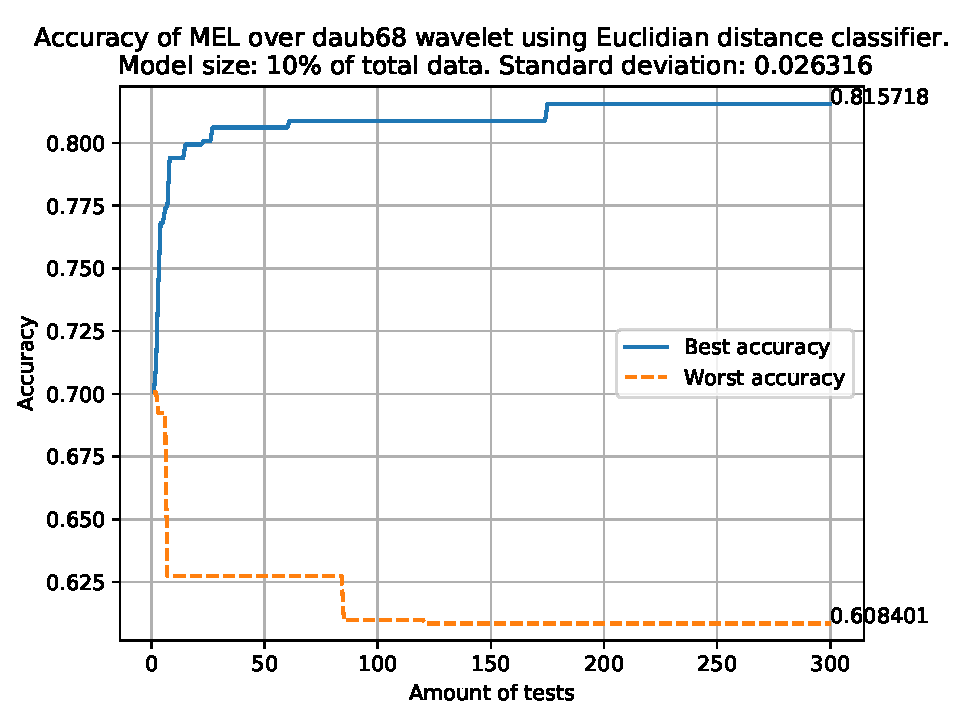
\includegraphics[scale=.8]{images/results/confusionMatrices/classifier_Euclidian_10.pdf}
			\caption{Accuracy \textit{x} number of tests - Euclidean distance with $M=10\%$}
			\label{fig:classifiereuclidian10}
		\end{figure}
		\begin{figure}[H]
			\centering
			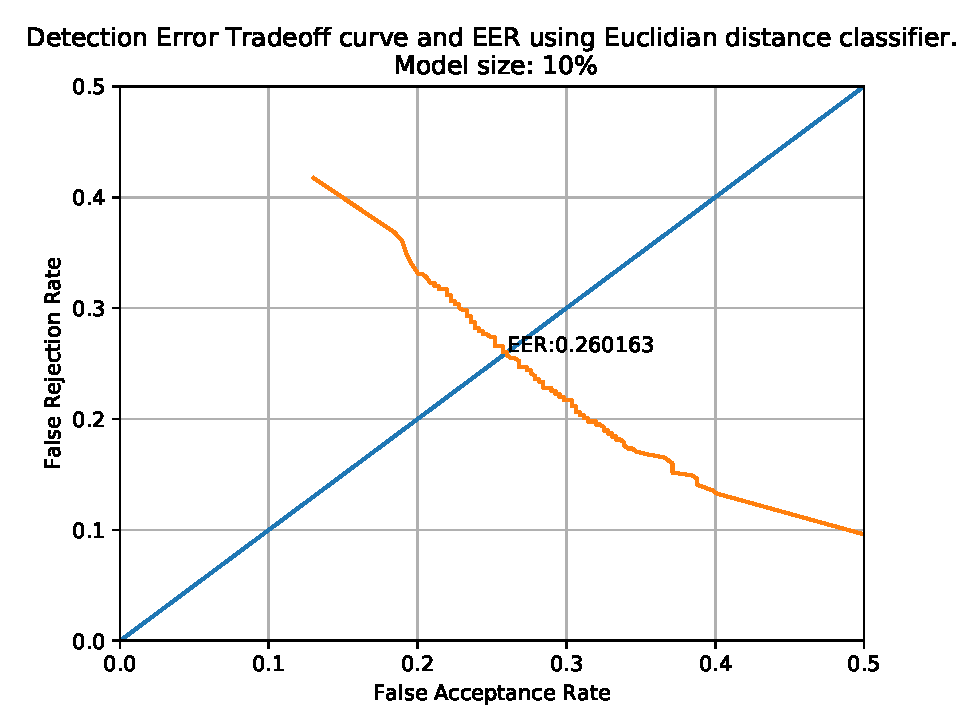
\includegraphics[scale=.8]{images/results/det/DET_for_classifier_Euclidian_10.pdf}
			\caption{DET curve of Euclidean distance results with $M=10\%$}
			\label{fig:detforclassifiereuclidian10}
		\end{figure}
	
		\begin{figure}[H]
			\centering
			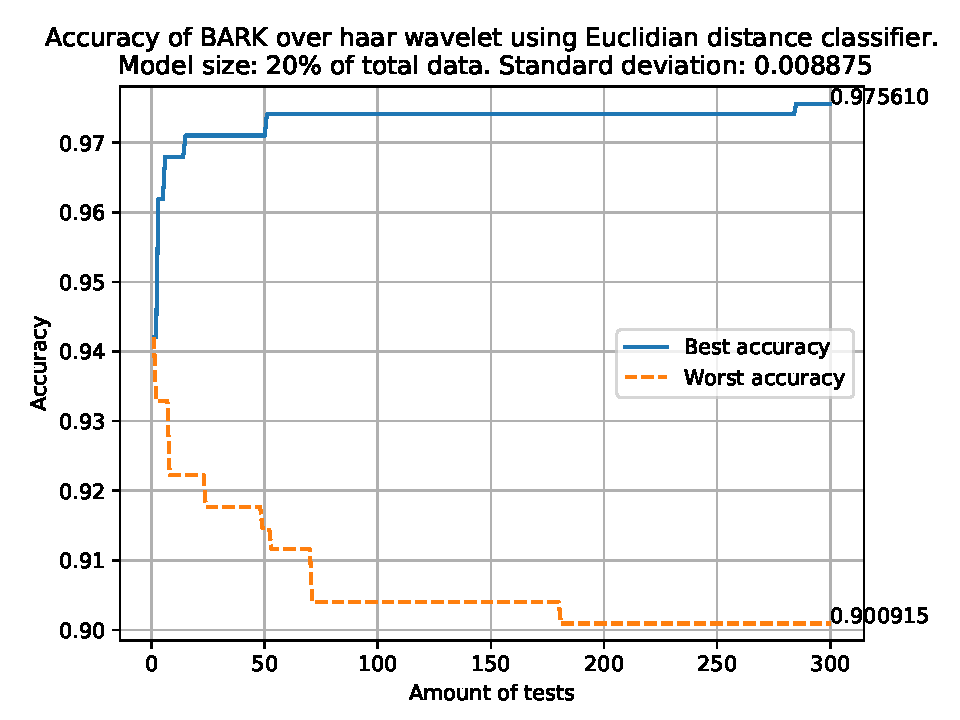
\includegraphics[scale=.8]{images/results/confusionMatrices/classifier_Euclidian_20.pdf}
			\caption{Accuracy \textit {x} number of tests - Euclidean distance with $M=20\%$}
			\label{fig:classifiereuclidian20}
		\end{figure}
		\begin{figure}[H]
			\centering
			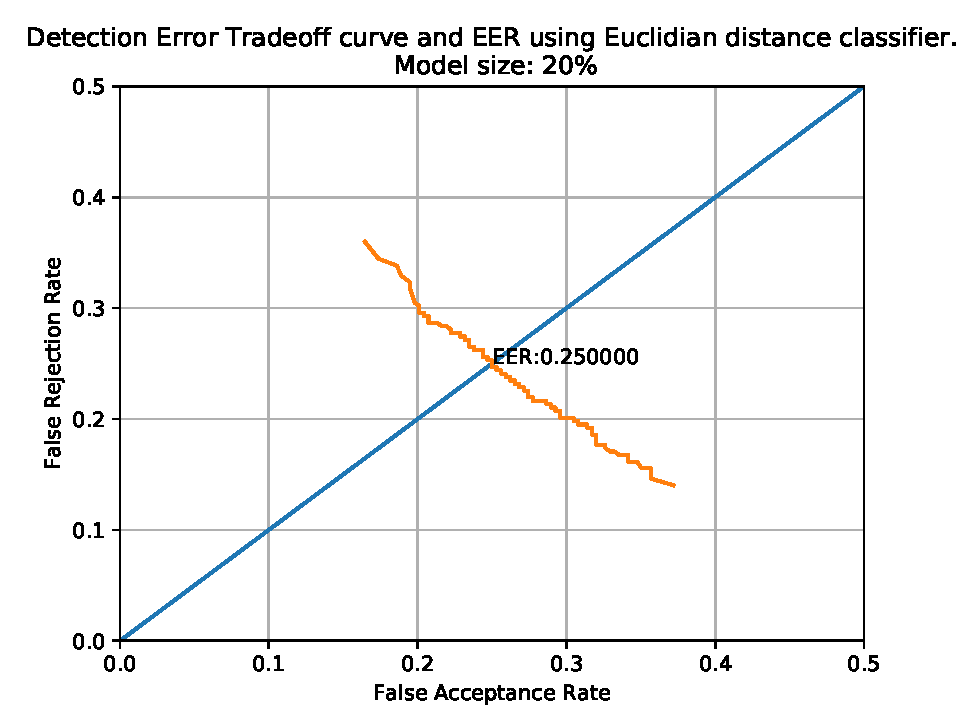
\includegraphics[scale=.8]{images/results/det/DET_for_classifier_Euclidian_20.pdf}
			\caption{DET curve of Euclidean distance results with $M=20\%$}
			\label{fig:detforclassifiereuclidian20}
		\end{figure}
	
	
		\begin{figure}[H]
			\centering
			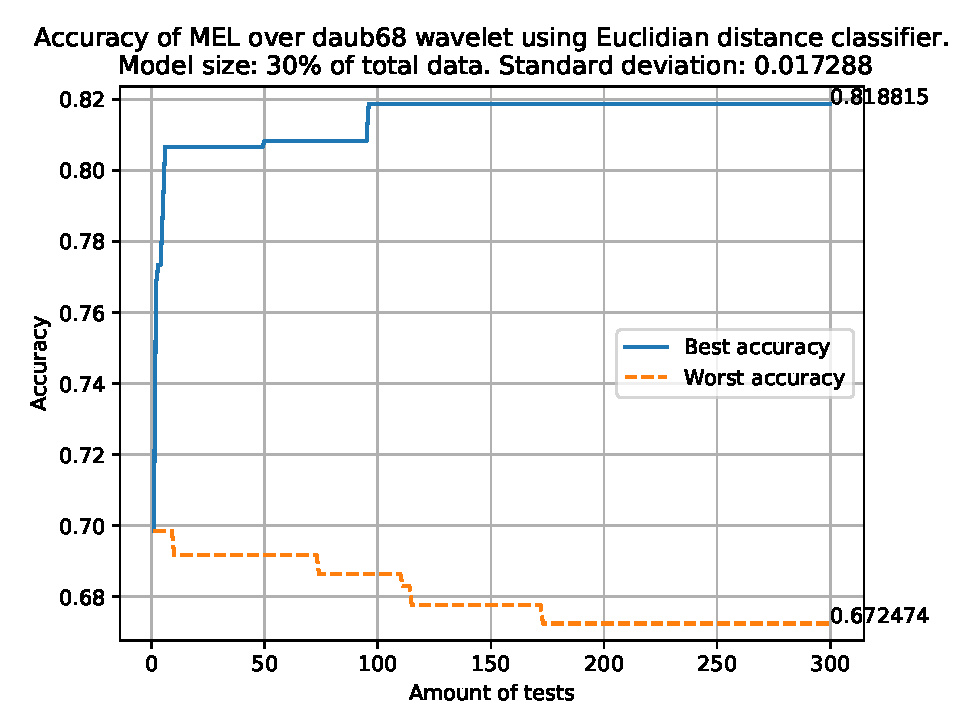
\includegraphics[scale=.8]{images/results/confusionMatrices/classifier_Euclidian_30.pdf}
			\caption{Accuracy \textit{x} number of tests - Euclidean distance with $M=30\%$}
			\label{fig:classifiereuclidian30}
		\end{figure}
		\begin{figure}[H]
			\centering
			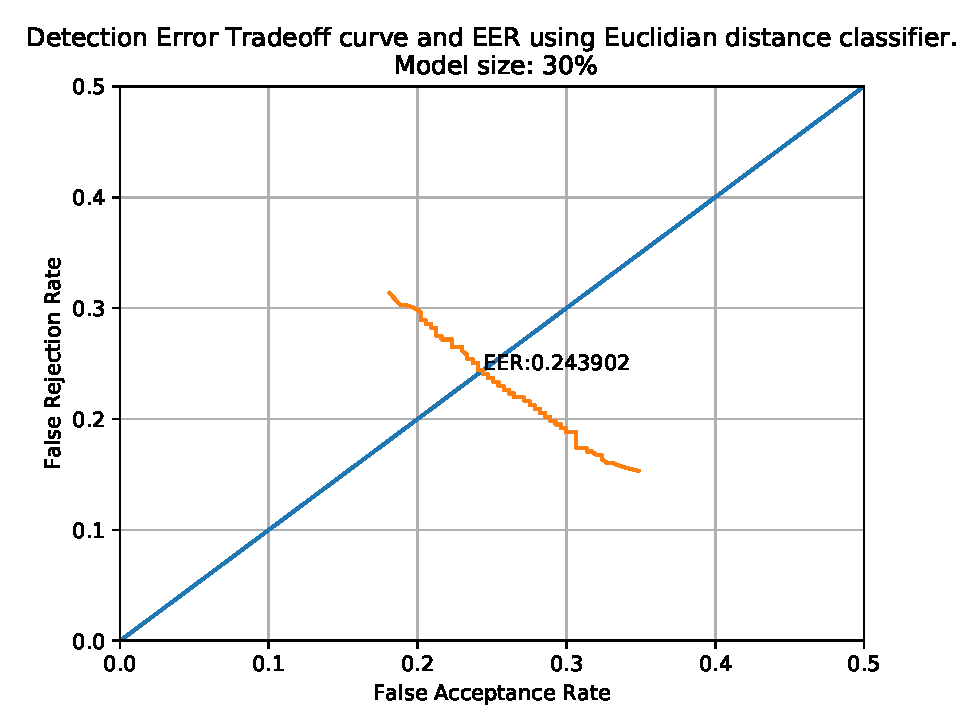
\includegraphics[scale=.8]{images/results/det/DET_for_classifier_Euclidian_30.pdf}
			\caption{DET curve of Euclidean distance results with $M=30\%$}
			\label{fig:detforclassifiereuclidian30}
		\end{figure}
	
	
		\begin{figure}[H]
			\centering
			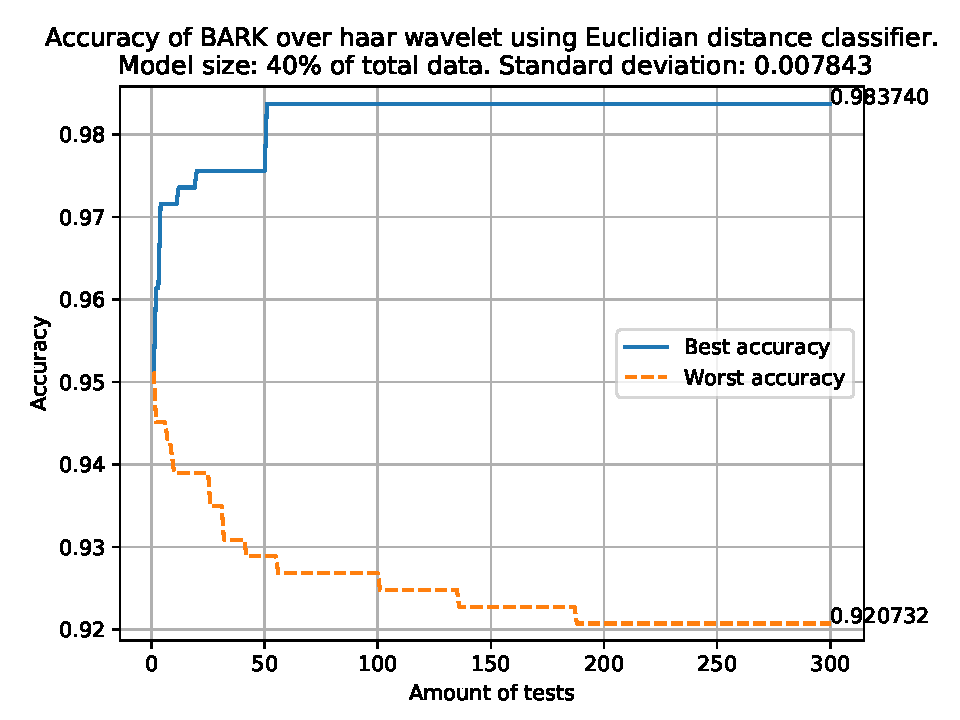
\includegraphics[scale=.8]{images/results/confusionMatrices/classifier_Euclidian_40.pdf}
			\caption{Accuracy \textit{X} number of tests - Euclidean distance with $M=40\%$}
			\label{fig:classifiereuclidian40}
		\end{figure}
		\begin{figure}[H]
			\centering
			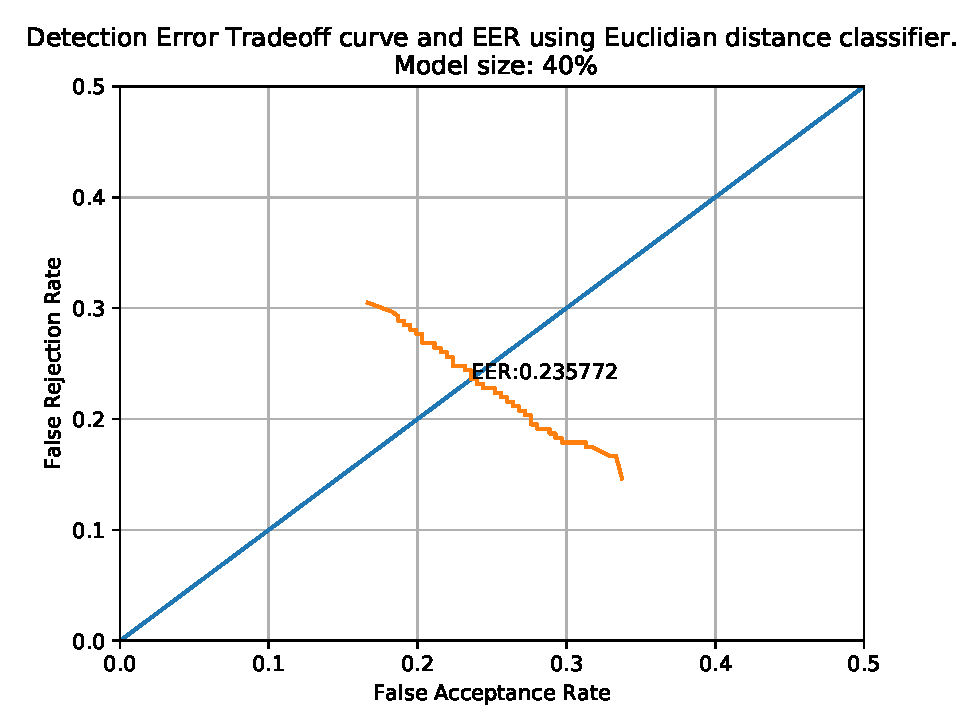
\includegraphics[scale=.8]{images/results/det/DET_for_classifier_Euclidian_40.pdf}
			\caption{DET curve of Euclidean distance results with $M=40\%$}
			\label{fig:detforclassifiereuclidian40}
		\end{figure}
	
	
		\begin{figure}[H]
			\centering
			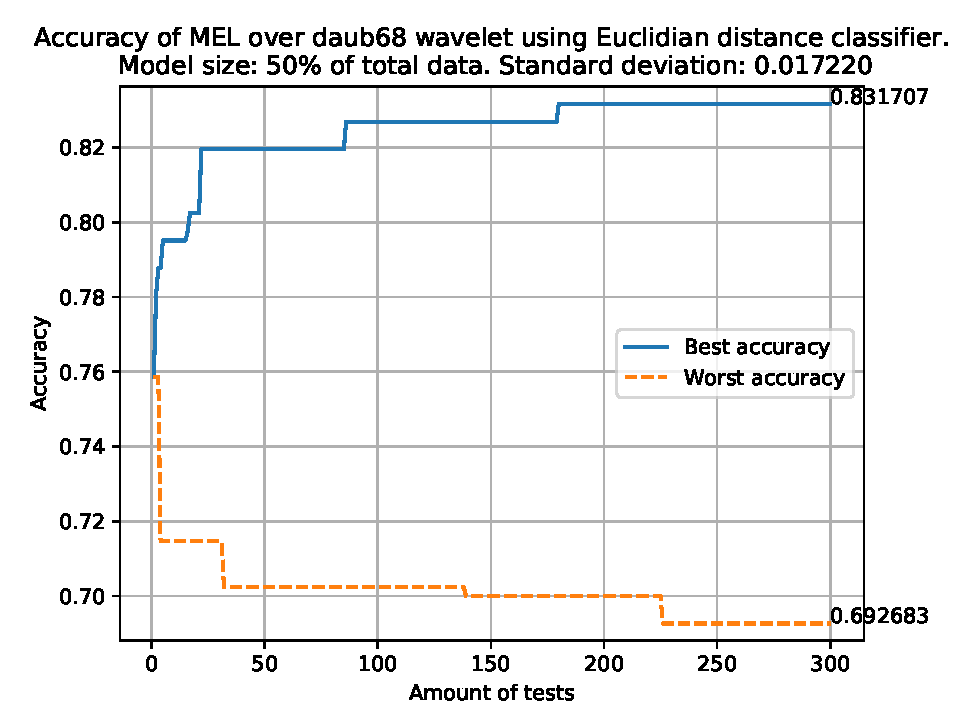
\includegraphics[scale=.8]{images/results/confusionMatrices/classifier_Euclidian_50.pdf}
			\caption{Accuracy \textit{x} number of tests - Euclidean distance with $M=50\%$}
			\label{fig:classifiereuclidian50}
		\end{figure}
		\begin{figure}[H]
			\centering
			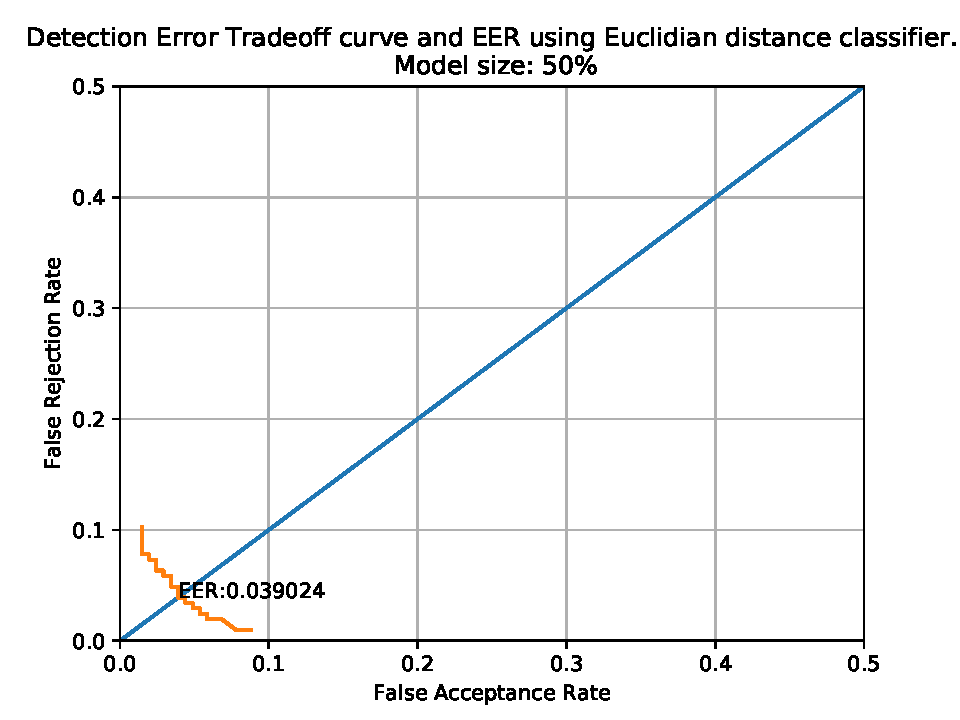
\includegraphics[scale=.8]{images/results/det/DET_for_classifier_Euclidian_50.pdf}
			\caption{DET curve of Euclidean distance results with $M=50\%$}
			\label{fig:detforclassifiereuclidian50}
		\end{figure}
	
	
		\begin{figure}[H]
			\centering
			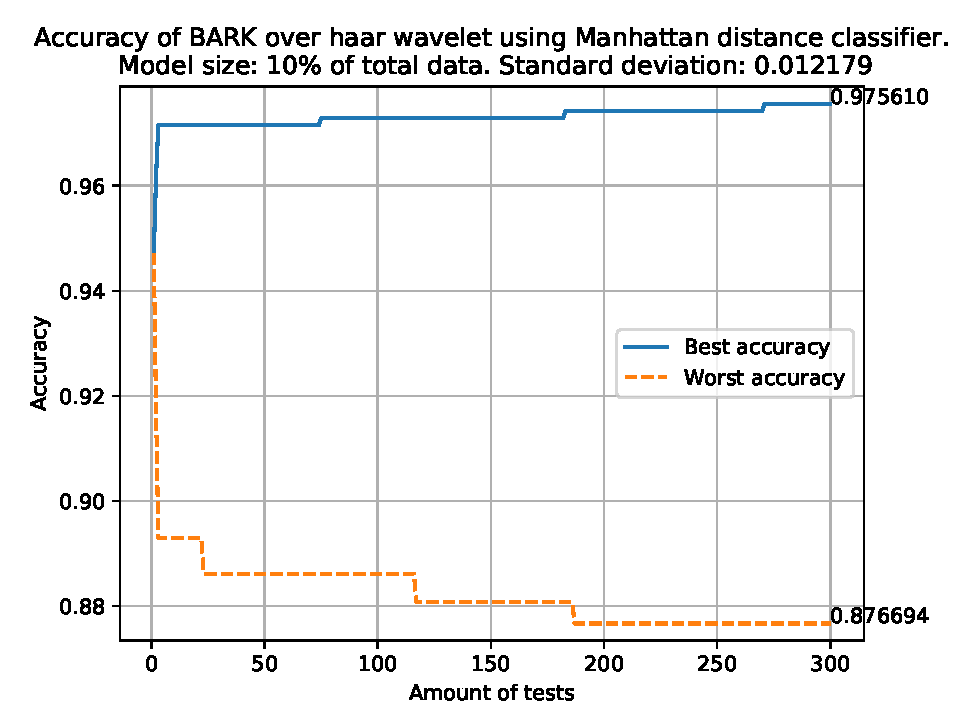
\includegraphics[scale=.8]{images/results/confusionMatrices/classifier_Manhattan_10.pdf}
			\caption{Accuracy \textit{x} number of tests - Manhattan distance with $M=10\%$}
			\label{fig:classifiermanhattan10}
		\end{figure}
		\begin{figure}[H]
			\centering
			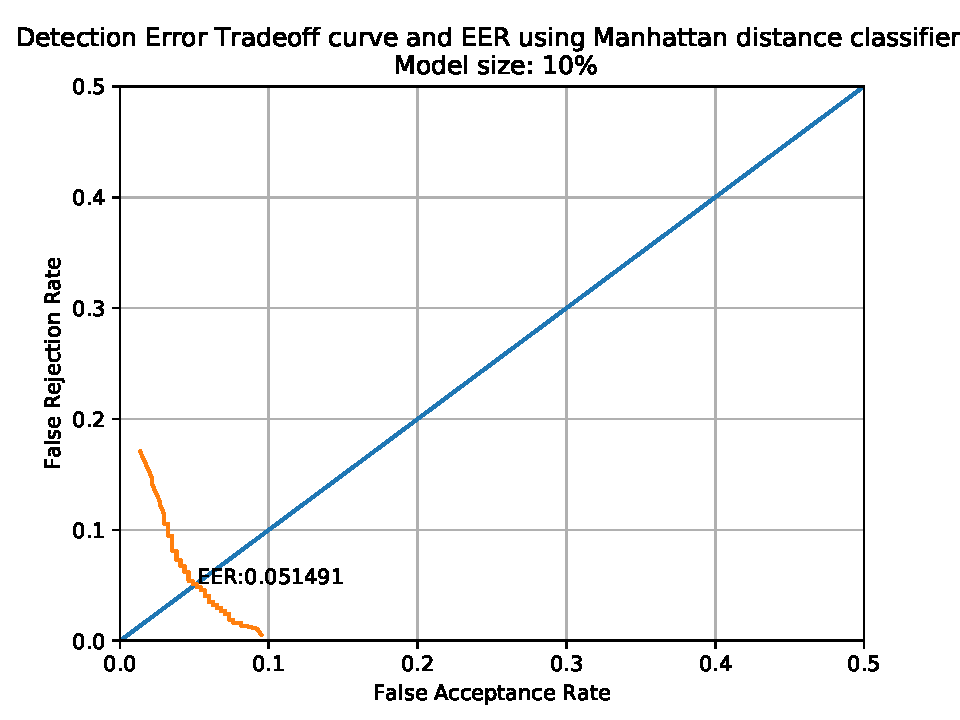
\includegraphics[scale=.8]{images/results/det/DET_for_classifier_Manhattan_10.pdf}
			\caption{DET curve of Manhattan distance results with $M=10\%$}
			\label{fig:detforclassifiermanhattan10}
		\end{figure}
	
	
		\begin{figure}[H]
			\centering
			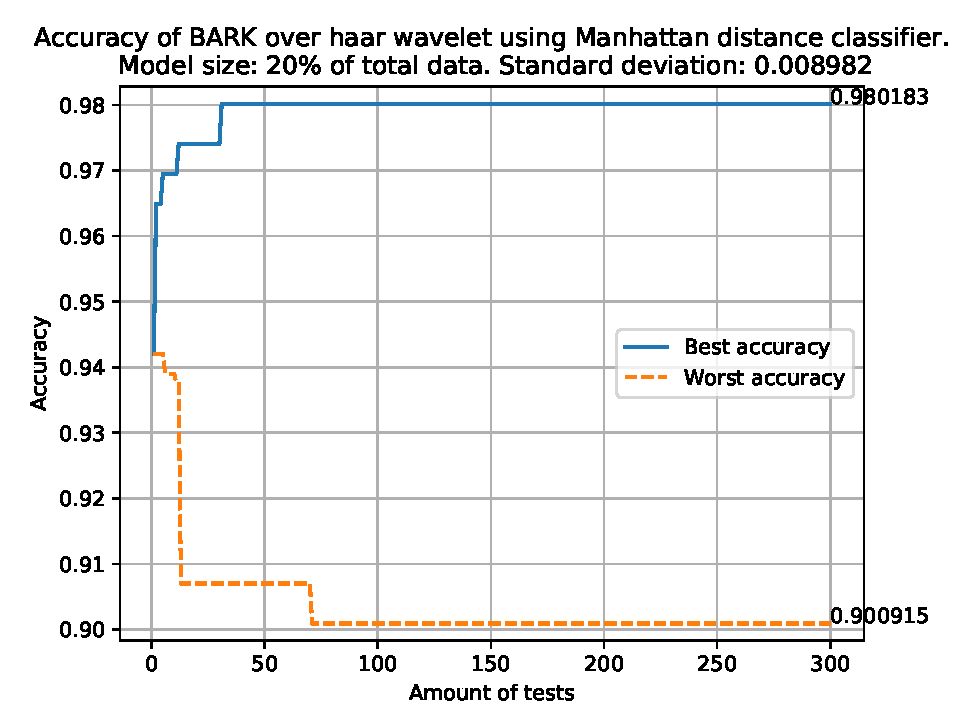
\includegraphics[scale=.8]{images/results/confusionMatrices/classifier_Manhattan_20.pdf}
			\caption{Accuracy \textit{x} number of tests - Manhattan distance with $M=20\%$}
			\label{fig:classifiermanhattan20}
		\end{figure}
		\begin{figure}[H]
			\centering
			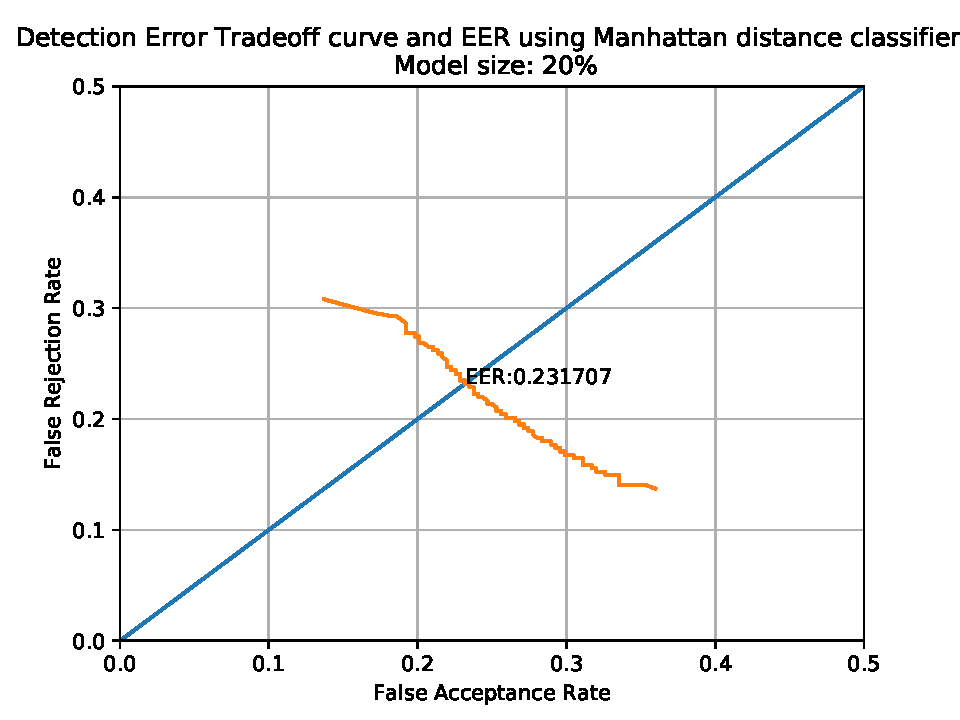
\includegraphics[scale=.8]{images/results/det/DET_for_classifier_Manhattan_20.pdf}
			\caption{DET curve of Manhattan distance with $M=20\%$}
			\label{fig:detforclassifiermanhattan20}
		\end{figure}
	
	
		 \begin{figure}[H]
			\centering
			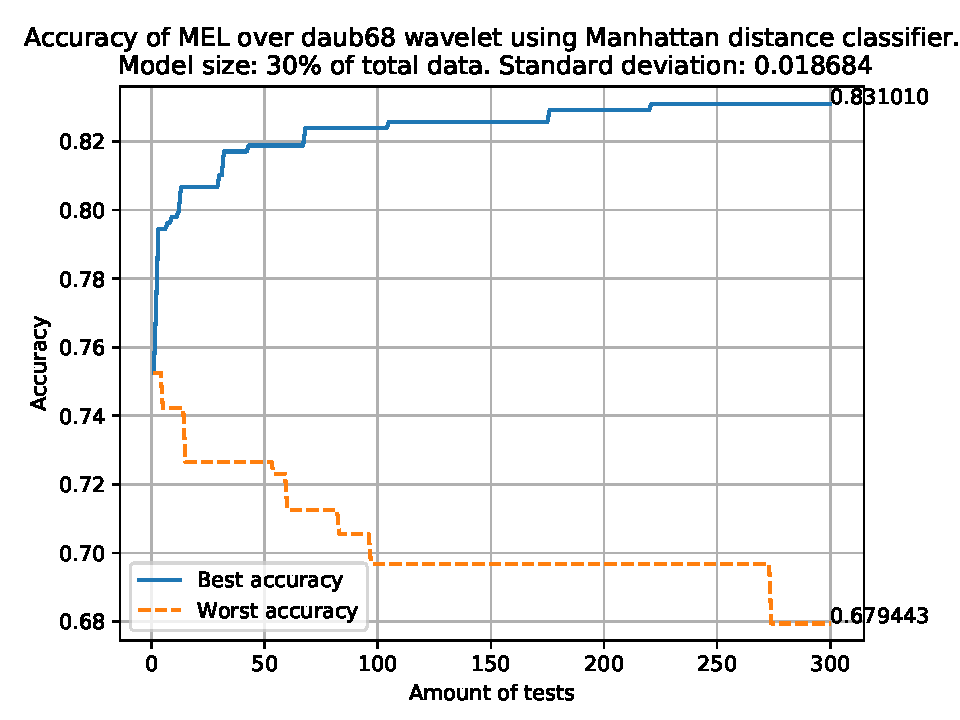
\includegraphics[scale=.8]{images/results/confusionMatrices/classifier_Manhattan_30.pdf}
			\caption{Accuracy \textit{x} number of tests - Manhattan distance with $M=30\%$}
			\label{fig:classifiermanhattan30}
		\end{figure}
		\begin{figure}[H]
			\centering
			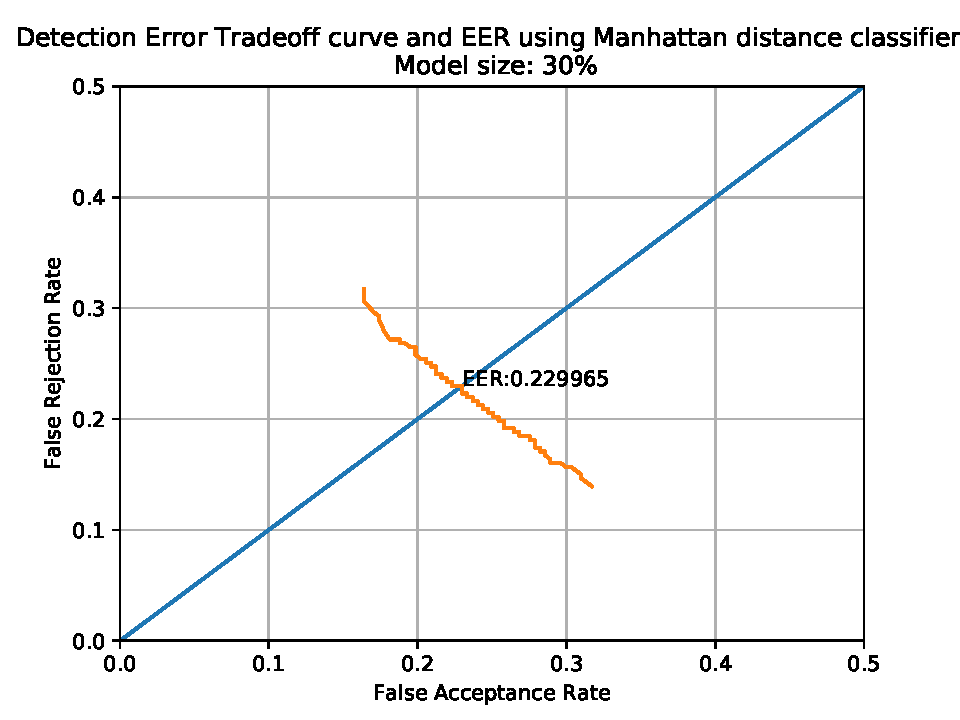
\includegraphics[scale=.8]{images/results/det/DET_for_classifier_Manhattan_30.pdf}
			\caption{DET curve of Manhattan distance with $M=30\%$}
			\label{fig:detforclassifiermanhattan30}
		\end{figure}
	
	
		\begin{figure}[H]
			\centering
			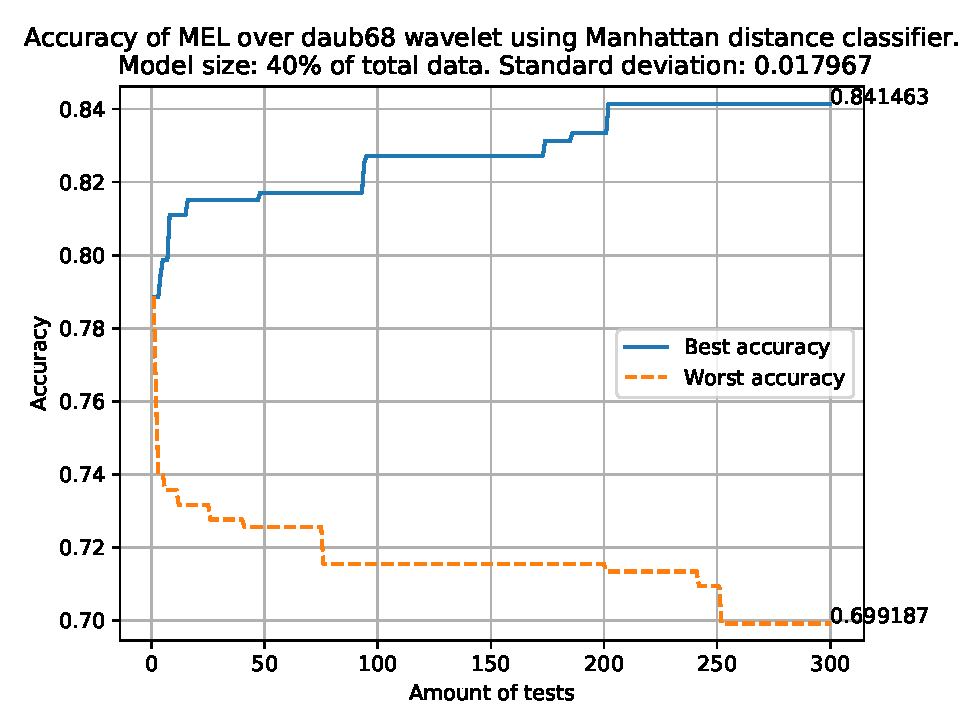
\includegraphics[scale=.8]{images/results/confusionMatrices/classifier_Manhattan_40.pdf}
			\caption{Accuracy \textit{x} number of tests - Manhattan distance with $M=40\%$}
			\label{fig:classifiermanhattan40}
		\end{figure}
		\begin{figure}[H]
			\centering
			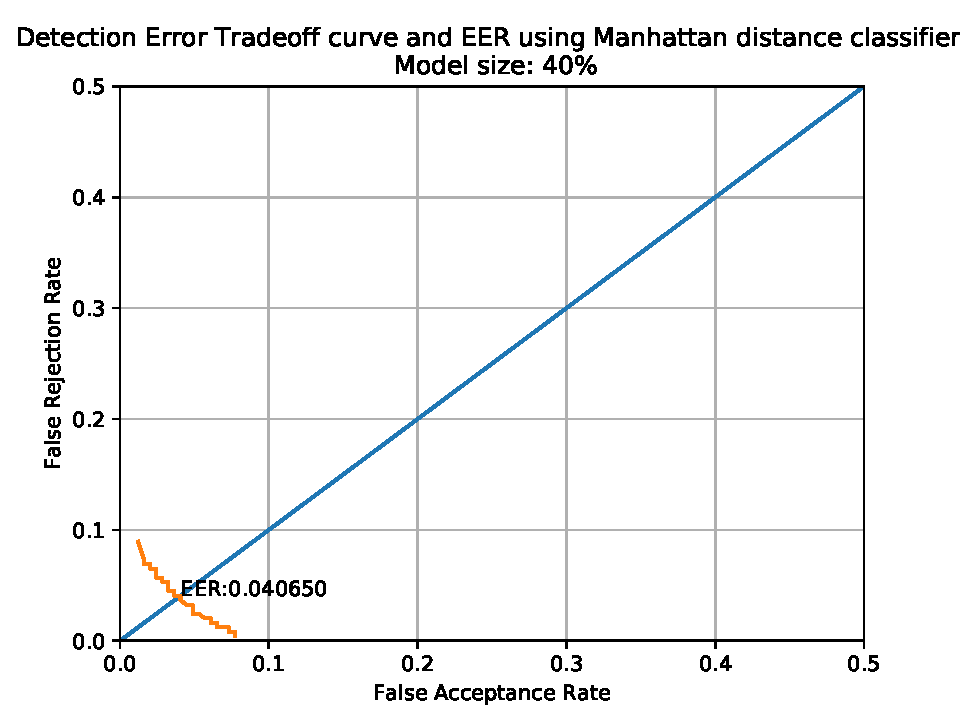
\includegraphics[scale=.8]{images/results/det/DET_for_classifier_Manhattan_40.pdf}
			\caption{DET curve of Manhattan distance results with $M=40\%$}
			\label{fig:detforclassifiermanhattan40}
		\end{figure}
	
	
		\begin{figure}[H]
			\centering
			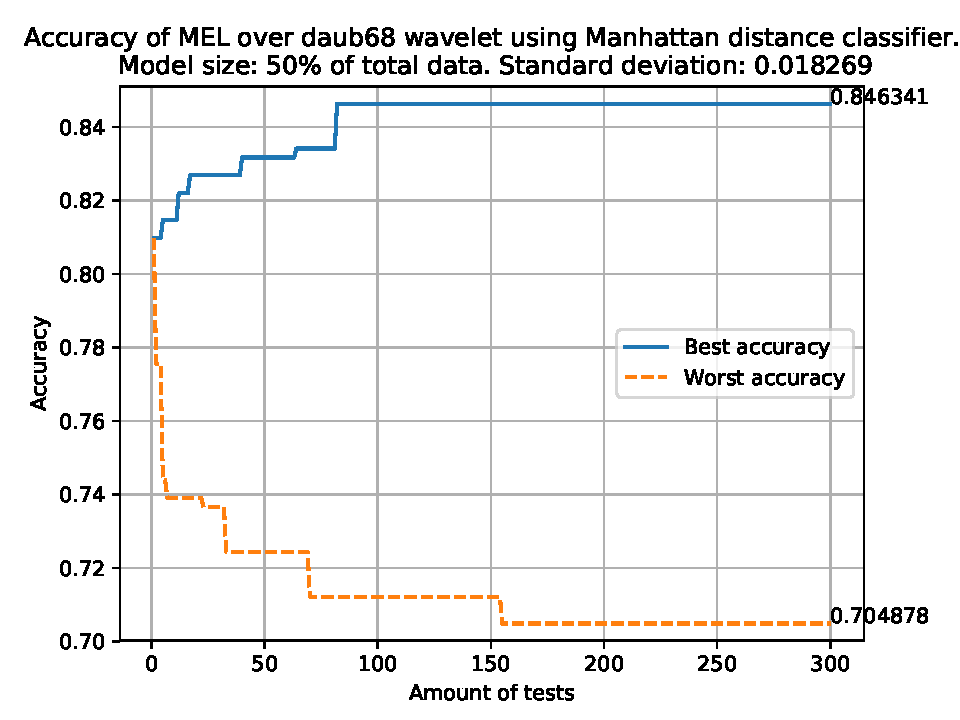
\includegraphics[scale=.8]{images/results/confusionMatrices/classifier_Manhattan_50.pdf}
			\caption{Accuracy \textit{x} number of tests - Manhattan distance with $M=50\%$}
			\label{fig:classifiermanhattan50}
		\end{figure}
		\begin{figure}[H]
			\centering
			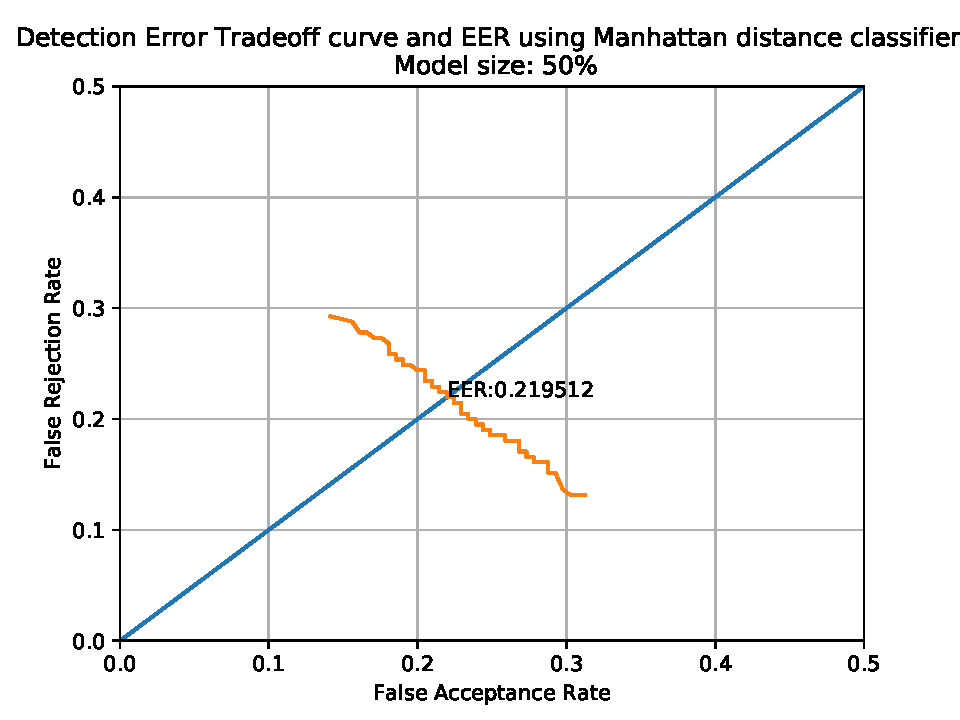
\includegraphics[scale=.8]{images/results/det/DET_for_classifier_Manhattan_50.pdf}
			\caption{DET curve of Manhattan distance results with $M=50\%$}
			\label{fig:detforclassifiermanhattan50}
		\end{figure}
	

\par Looking at the Tables from \ref{tab:experiment02ResultsEuclidian} to \ref{tab:classifier_Manhattan_50_worse}, we can observe the \textbf{best value} of accuracy and EER: \textbf{0.885366 and 0.165854} for the Euclidean distance classifier, and \textbf{0.897561 and 0.156098} for the Manhattan distance classifier. Thus, there is no practical difference when comparing the \textit{pattern-matching} metric criteria used. In addition, we can state that a relatively high level of accuracy was obtained, assuming the classifier modesty.
\\
\par Once again, considering the combination \textbf{Haar+Bark}, we explore hereafter the \textbf{maximum value of accuracy and minimum EER} that can be achieved with an SVM. The corresponding results are shown in Table \ref{tab:experiment03Results} and, additional details can be found in Tables \ref{tab:classifier_SVM_10_best}, \ref{tab:classifier_SVM_10_worse}, \ref{tab:classifier_SVM_20_best}, \ref{tab:classifier_SVM_20_worse}, \ref{tab:classifier_SVM_30_best}, \ref{tab:classifier_SVM_30_worse}, \ref{tab:classifier_SVM_40_best}, \ref{tab:classifier_SVM_40_worse}, \ref{tab:classifier_SVM_50_best}, and \ref{tab:classifier_SVM_50_worse}. As a complement, Figures \ref{fig:classifiersvm10}, \ref{fig:detsvm10}, \ref{fig:classifiersvm20}, \ref{fig:detsvm20}, \ref{fig:classifiersvm30}, \ref{fig:detsvm30}, \ref{fig:classifiersvm40}, \ref{fig:detsvm40}, \ref{fig:classifiersvm50}, and \ref{fig:detsvm50} show the corresponding plots.\\
\begin{table}[H]
	\newcommand{\mc}[3]{\multicolumn{#1}{#2}{#3}}
	\definecolor{tcA}{rgb}{0.65098,0.65098,0.65098}
	\definecolor{tcB}{rgb}{0.447059,0.74902,0.266667}
	\begin{center}
		\caption{Resultados da abordagem com SVM}
		\begin{tabular}{|p{0.15\linewidth}|p{0.11\linewidth}|p{0.11\linewidth}|p{0.11\linewidth}|p{0.14\linewidth}|p{0.14\linewidth}|}\hline
			% use packages: color,colortbl
			\rowcolor{tcA}
			\centering\textbf{$M$} & \centering\textbf{Acurácia mínima} & \centering\textbf{Acurácia máxima} & \centering\textbf{Média das acurácias} & \centering\textbf{Desvio padrão da acurácia} & \begin{center}\textbf{EER}\end{center}\\\hline
			
			\rowcolor{tcB}
			% Loads data from tables/results/paraconsistentPlane/distParacomFrom10.csv
			\csvreader[
			late after line=\\\hline\rowcolor{tcB},%
			separator=comma,
			]{tables/results/experiment02ResultsSVM.csv}{1=\eme,2=\minAccu,3=\maxAccu,4=\meanAccu,5=\stdDev,6=\eer}{\centering\eme\% & \centering\StrSubstitute[0]{\minAccu}{.}{,} & \centering\StrSubstitute[0]{\maxAccu}{.}{,} & \centering\StrSubstitute[0]{\meanAccu}{.}{,} & \centering\StrSubstitute[0]{\stdDev}{.}{,} & \StrSubstitute[0]{\eer}{.}{,}}
			
		\end{tabular}
		\label{tab:experiment03Results}
		\\Fonte: Elaborado pelo autor, 2021.
	\end{center}
\end{table}

\begin{table}[h]
\newcommand{\mc}[3]{\multicolumn{#1}{#2}{#3}}
\definecolor{tcB}{rgb}{0.447059,0.74902,0.266667}
\definecolor{tcC}{rgb}{0,0,0}
\definecolor{tcD}{rgb}{0,0.4,0.701961}
\definecolor{tcA}{rgb}{0.65098,0.65098,0.65098}
\begin{center}
	\begin{tabular}{ccc}
		% use packages: color,colortbl
		\mc{1}{l}{} & \mc{1}{>{\columncolor{tcA}}c}{\textbf{Verdadeiro}} & \mc{1}{>{\columncolor{tcA}}c}{\textbf{Falso}}\\

		\mc{1}{>{\columncolor{tcA}}r}{\textbf{Verdadeiro}} & \mc{1}{>{\columncolor{tcB}}c}{\textcolor{tcC}{339}} & \mc{1}{>{\columncolor{tcD}}c}{\textcolor{tcC}{24}}\\

		\mc{1}{>{\columncolor{tcA}}r}{\textbf{Falso}} & \mc{1}{>{\columncolor{tcD}}c}{\textcolor{tcC}{30}} & \mc{1}{>{\columncolor{tcB}}c}{\textcolor{tcC}{345}}
	\end{tabular}
	\caption{Melhor tabela de confusão para classificador SVM 10\%}
	\label{tab:classifier_SVM_10_best}
\end{center}
\end{table}

\begin{table}[h]
	\newcommand{\mc}[3]{\multicolumn{#1}{#2}{#3}}
	\definecolor{tcB}{rgb}{0.447059,0.74902,0.266667}
	\definecolor{tcC}{rgb}{0,0,0}
	\definecolor{tcD}{rgb}{0,0.4,0.701961}
	\definecolor{tcA}{rgb}{0.65098,0.65098,0.65098}
	\begin{center}
		\begin{tabular}{ccc}
			% use packages: color,colortbl
			\mc{1}{l}{} & \mc{1}{>{\columncolor{tcA}}c}{\textbf{Verdadeiro}} & \mc{1}{>{\columncolor{tcA}}c}{\textbf{Falso}}\\
			
			\mc{1}{>{\columncolor{tcA}}r}{\textbf{Verdadeiro}} & \mc{1}{>{\columncolor{tcB}}c}{\textcolor{tcC}{329}} & \mc{1}{>{\columncolor{tcD}}c}{\textcolor{tcC}{93}}\\
			
			\mc{1}{>{\columncolor{tcA}}r}{\textbf{Falso}} & \mc{1}{>{\columncolor{tcD}}c}{\textcolor{tcC}{40}} & \mc{1}{>{\columncolor{tcB}}c}{\textcolor{tcC}{276}}
		\end{tabular}
		\caption{Pior tabela de confusão para classificador SVM 10\%}
		\label{tab:classifier_SVM_10_worse}
	\end{center}
\end{table}

\begin{table}[h] 					\newcommand{\mc}[3]{\multicolumn{#1}{#2}{#3}} 					\definecolor{tcB}{rgb}{0.447059,0.74902,0.266667} 					\definecolor{tcC}{rgb}{0,0,0} 					\definecolor{tcD}{rgb}{0,0.5,1} 					\definecolor{tcA}{rgb}{0.65098,0.65098,0.65098} 					\begin{center} 						\subfloat[Best confusion matrix]{ 							\begin{tabular}{ccc} 								\mc{1}{l}{} & \mc{1}{>{\columncolor{tcA}}c}{\textbf{genuine}} & \mc{1}{>{\columncolor{tcA}}c}{\textbf{spoofed}}\\ 								\mc{1}{>{\columncolor{tcA}}r}{\textbf{genuine}} & \mc{1}{>{\columncolor{tcB}}c}{\textcolor{tcC}{306}} & \mc{1}{>{\columncolor{tcD}}c}{\textcolor{tcC}{29}}\\ 								\mc{1}{>{\columncolor{tcA}}r}{\textbf{spoofed}} & \mc{1}{>{\columncolor{tcD}}c}{\textcolor{tcC}{22}} & \mc{1}{>{\columncolor{tcB}}c}{\textcolor{tcC}{299}} 							\end{tabular} 							\label{tab:classifier_Euclidian_10_best} 						} 						\qquad 						\subfloat[Worst confusion matrix]{ 							\begin{tabular}{ccc} 								\mc{1}{l}{} & \mc{1}{>{\columncolor{tcA}}c}{\textbf{genuine}} & \mc{1}{>{\columncolor{tcA}}c}{\textbf{spoofed}}\\ 								\mc{1}{>{\columncolor{tcA}}r}{\textbf{genuine}} & \mc{1}{>{\columncolor{tcB}}c}{\textcolor{tcC}{255}} & \mc{1}{>{\columncolor{tcD}}c}{\textcolor{tcC}{56}}\\ 								\mc{1}{>{\columncolor{tcA}}r}{\textbf{spoofed}} & \mc{1}{>{\columncolor{tcD}}c}{\textcolor{tcC}{73}} & \mc{1}{>{\columncolor{tcB}}c}{\textcolor{tcC}{272}} 							\end{tabular} 							\label{tab:classifier_Euclidian_10_worse} 						} 					\end{center} 					\caption{Confusion matrices for SVM classifier at 20\% model} 				\end{table}
\begin{table}[h] 					\newcommand{\mc}[3]{\multicolumn{#1}{#2}{#3}} 					\definecolor{tcB}{rgb}{0.447059,0.74902,0.266667} 					\definecolor{tcC}{rgb}{0,0,0} 					\definecolor{tcD}{rgb}{0,0.5,1} 					\definecolor{tcA}{rgb}{0.65098,0.65098,0.65098} 					\begin{center} 						\subfloat[Best confusion matrix]{ 							\begin{tabular}{ccc} 								\mc{1}{l}{} & \mc{1}{>{\columncolor{tcA}}c}{\textbf{genuine}} & \mc{1}{>{\columncolor{tcA}}c}{\textbf{spoofed}}\\ 								\mc{1}{>{\columncolor{tcA}}r}{\textbf{genuine}} & \mc{1}{>{\columncolor{tcB}}c}{\textcolor{tcC}{272}} & \mc{1}{>{\columncolor{tcD}}c}{\textcolor{tcC}{27}}\\ 								\mc{1}{>{\columncolor{tcA}}r}{\textbf{spoofed}} & \mc{1}{>{\columncolor{tcD}}c}{\textcolor{tcC}{15}} & \mc{1}{>{\columncolor{tcB}}c}{\textcolor{tcC}{260}} 							\end{tabular} 							\label{tab:classifier_Euclidian_10_best} 						} 						\qquad 						\subfloat[Worst confusion matrix]{ 							\begin{tabular}{ccc} 								\mc{1}{l}{} & \mc{1}{>{\columncolor{tcA}}c}{\textbf{genuine}} & \mc{1}{>{\columncolor{tcA}}c}{\textbf{spoofed}}\\ 								\mc{1}{>{\columncolor{tcA}}r}{\textbf{genuine}} & \mc{1}{>{\columncolor{tcB}}c}{\textcolor{tcC}{233}} & \mc{1}{>{\columncolor{tcD}}c}{\textcolor{tcC}{39}}\\ 								\mc{1}{>{\columncolor{tcA}}r}{\textbf{spoofed}} & \mc{1}{>{\columncolor{tcD}}c}{\textcolor{tcC}{54}} & \mc{1}{>{\columncolor{tcB}}c}{\textcolor{tcC}{248}} 							\end{tabular} 							\label{tab:classifier_Euclidian_10_worse} 						} 					\end{center} 					\caption{Confusion matrices for SVM classifier at 30\% model} 				\end{table}
\begin{table}[h]
\newcommand{\mc}[3]{\multicolumn{#1}{#2}{#3}}
\definecolor{tcB}{rgb}{0.447059,0.74902,0.266667}
\definecolor{tcC}{rgb}{0,0,0}
\definecolor{tcD}{rgb}{0,0.5,1}
\definecolor{tcA}{rgb}{0.65098,0.65098,0.65098}
\begin{center}
	\begin{tabular}{ccc}
		% use packages: color,colortbl
		\mc{1}{l}{} & \mc{1}{>{\columncolor{tcA}}c}{\textbf{Verdadeiro}} & \mc{1}{>{\columncolor{tcA}}c}{\textbf{Falso}}\\

		\mc{1}{>{\columncolor{tcA}}r}{\textbf{Verdadeiro}} & \mc{1}{>{\columncolor{tcB}}c}{\textcolor{tcC}{234}} & \mc{1}{>{\columncolor{tcD}}c}{\textcolor{tcC}{14}}\\

		\mc{1}{>{\columncolor{tcA}}r}{\textbf{Falso}} & \mc{1}{>{\columncolor{tcD}}c}{\textcolor{tcC}{12}} & \mc{1}{>{\columncolor{tcB}}c}{\textcolor{tcC}{232}}
	\end{tabular}
	\caption{Melhor tabela de confusão para classificador SVM 40\%}
	\label{tab:classifier_SVM_40_best}
\end{center}
\end{table}

\begin{table}[h]
	\newcommand{\mc}[3]{\multicolumn{#1}{#2}{#3}}
	\definecolor{tcB}{rgb}{0.447059,0.74902,0.266667}
	\definecolor{tcC}{rgb}{0,0,0}
	\definecolor{tcD}{rgb}{0,0.5,1}
	\definecolor{tcA}{rgb}{0.65098,0.65098,0.65098}
	\begin{center}
		\begin{tabular}{ccc}
			% use packages: color,colortbl
			\mc{1}{l}{} & \mc{1}{>{\columncolor{tcA}}c}{\textbf{Verdadeiro}} & \mc{1}{>{\columncolor{tcA}}c}{\textbf{Falso}}\\
			
			\mc{1}{>{\columncolor{tcA}}r}{\textbf{Verdadeiro}} & \mc{1}{>{\columncolor{tcB}}c}{\textcolor{tcC}{216}} & \mc{1}{>{\columncolor{tcD}}c}{\textcolor{tcC}{37}}\\
			
			\mc{1}{>{\columncolor{tcA}}r}{\textbf{Falso}} & \mc{1}{>{\columncolor{tcD}}c}{\textcolor{tcC}{30}} & \mc{1}{>{\columncolor{tcB}}c}{\textcolor{tcC}{209}}
		\end{tabular}
		\caption{Pior tabela de confusão para classificador SVM 40\%}
		\label{tab:classifier_SVM_40_worse}
	\end{center}
\end{table}

\begin{table}[h] 					\newcommand{\mc}[3]{\multicolumn{#1}{#2}{#3}} 					\definecolor{tcB}{rgb}{0.447059,0.74902,0.266667} 					\definecolor{tcC}{rgb}{0,0,0} 					\definecolor{tcD}{rgb}{0,0.5,1} 					\definecolor{tcA}{rgb}{0.65098,0.65098,0.65098} 					\begin{center} 						\subfloat[Best confusion matrix]{ 							\begin{tabular}{ccc} 								\mc{1}{l}{} & \mc{1}{>{\columncolor{tcA}}c}{\textbf{genuine}} & \mc{1}{>{\columncolor{tcA}}c}{\textbf{spoofed}}\\ 								\mc{1}{>{\columncolor{tcA}}r}{\textbf{genuine}} & \mc{1}{>{\columncolor{tcB}}c}{\textcolor{tcC}{205}} & \mc{1}{>{\columncolor{tcD}}c}{\textcolor{tcC}{1}}\\ 								\mc{1}{>{\columncolor{tcA}}r}{\textbf{spoofed}} & \mc{1}{>{\columncolor{tcD}}c}{\textcolor{tcC}{0}} & \mc{1}{>{\columncolor{tcB}}c}{\textcolor{tcC}{204}} 							\end{tabular} 							\label{tab:classifier_SVM_50_best} 						} 						\qquad 						\subfloat[Worst confusion matrix]{ 							\begin{tabular}{ccc} 								\mc{1}{l}{} & \mc{1}{>{\columncolor{tcA}}c}{\textbf{genuine}} & \mc{1}{>{\columncolor{tcA}}c}{\textbf{spoofed}}\\ 								\mc{1}{>{\columncolor{tcA}}r}{\textbf{genuine}} & \mc{1}{>{\columncolor{tcB}}c}{\textcolor{tcC}{196}} & \mc{1}{>{\columncolor{tcD}}c}{\textcolor{tcC}{17}}\\ 								\mc{1}{>{\columncolor{tcA}}r}{\textbf{spoofed}} & \mc{1}{>{\columncolor{tcD}}c}{\textcolor{tcC}{9}} & \mc{1}{>{\columncolor{tcB}}c}{\textcolor{tcC}{188}} 							\end{tabular} 							\label{tab:classifier_SVM_50_worse} 						} 					\end{center} 					\caption{Confusion matrices for SVM distance classifier at 50\% model} 				\end{table}
	\begin{figure}[H]
		\centering
		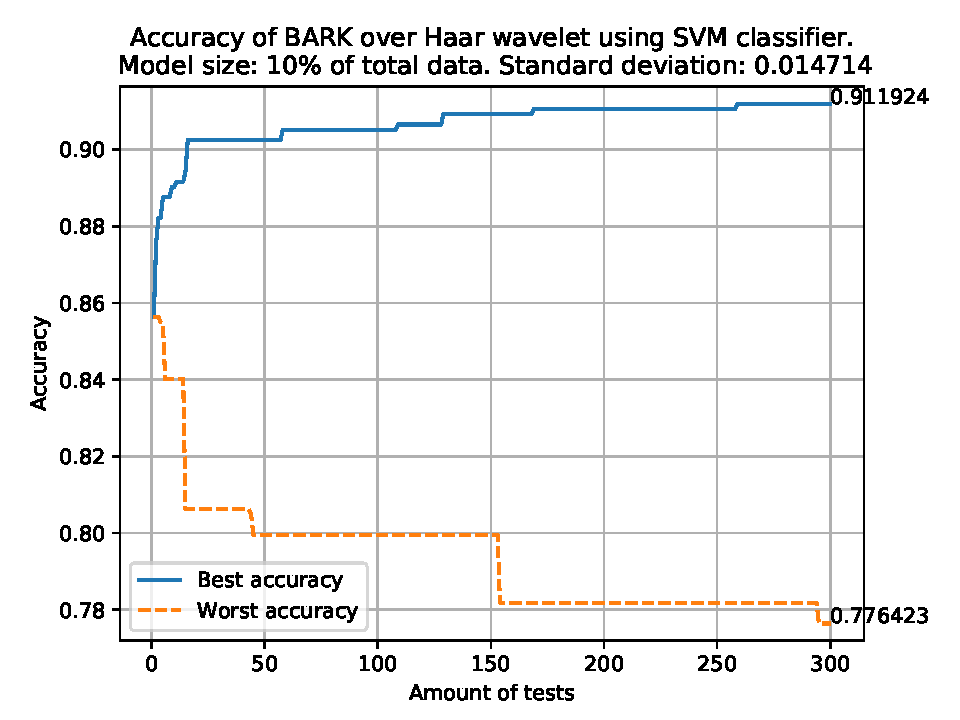
\includegraphics[scale=.8]{images/results/confusionMatrices/classifier_SVM_10.pdf}
		\caption{Accuracy \textit{x} number of tests - SVM with $M=10\%$}
		\label{fig:classifiersvm10}
	\end{figure}
	\begin{figure}[H]
		\centering
		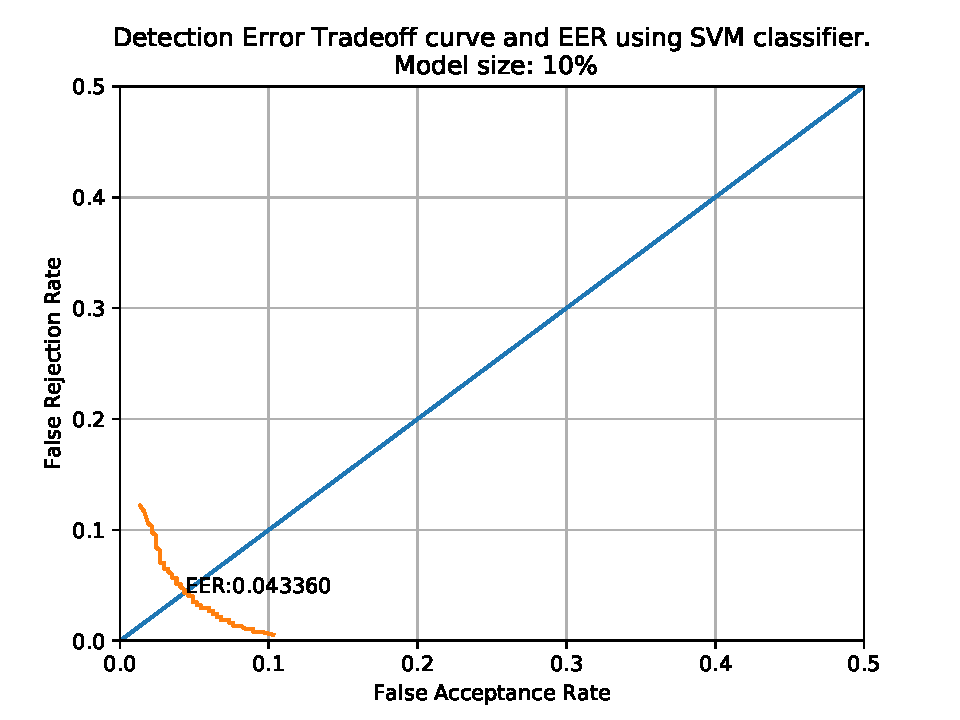
\includegraphics[scale=.8]{images/results/det/DET_for_classifier_SVM_10.pdf}
		\caption{DET curve of SVM results with $M=10\%$}
		\label{fig:detsvm10}
	\end{figure}
	\begin{figure}[H]
		\centering
		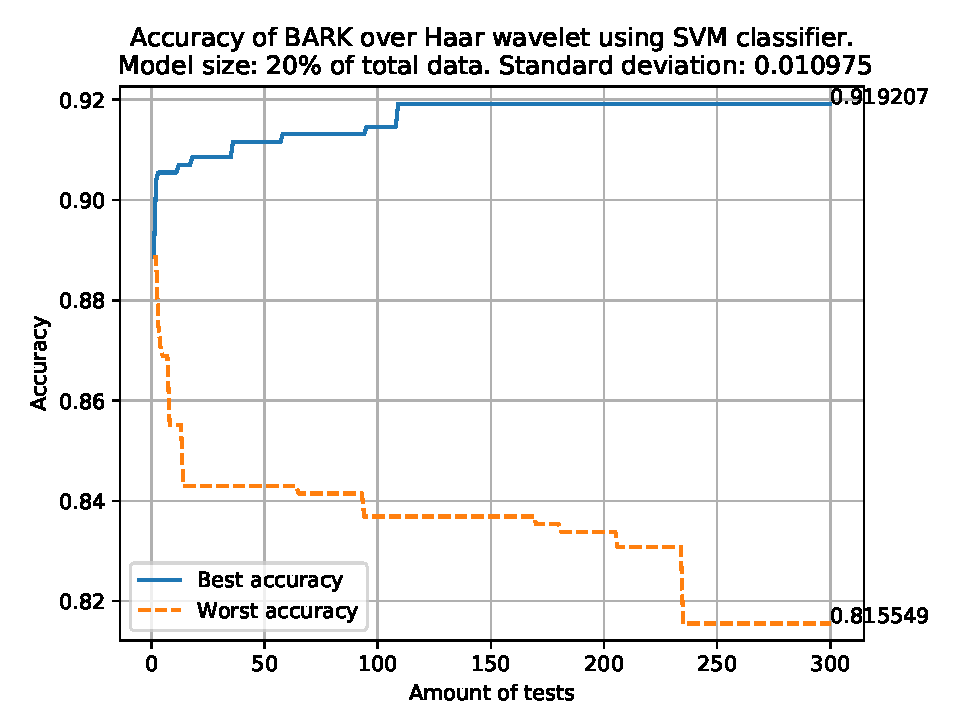
\includegraphics[scale=.8]{images/results/confusionMatrices/classifier_SVM_20.pdf}
		\caption{Accuracy \textit{x} number of tests - SVM with $M=20\%$}
		\label{fig:classifiersvm20}
	\end{figure}
	\begin{figure}[H]
		\centering
		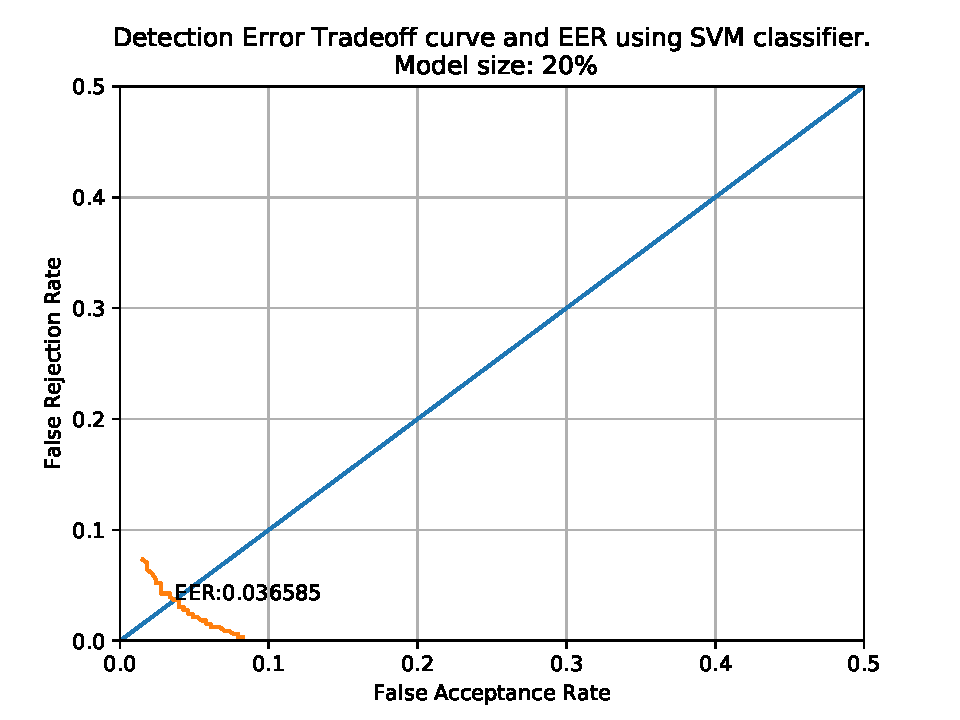
\includegraphics[scale=.8]{images/results/det/DET_for_classifier_SVM_20.pdf}
		\caption{DET curve of SVM results with $M=20\%$}
		\label{fig:detsvm20}
	\end{figure}
	\begin{figure}[H]
		\centering
		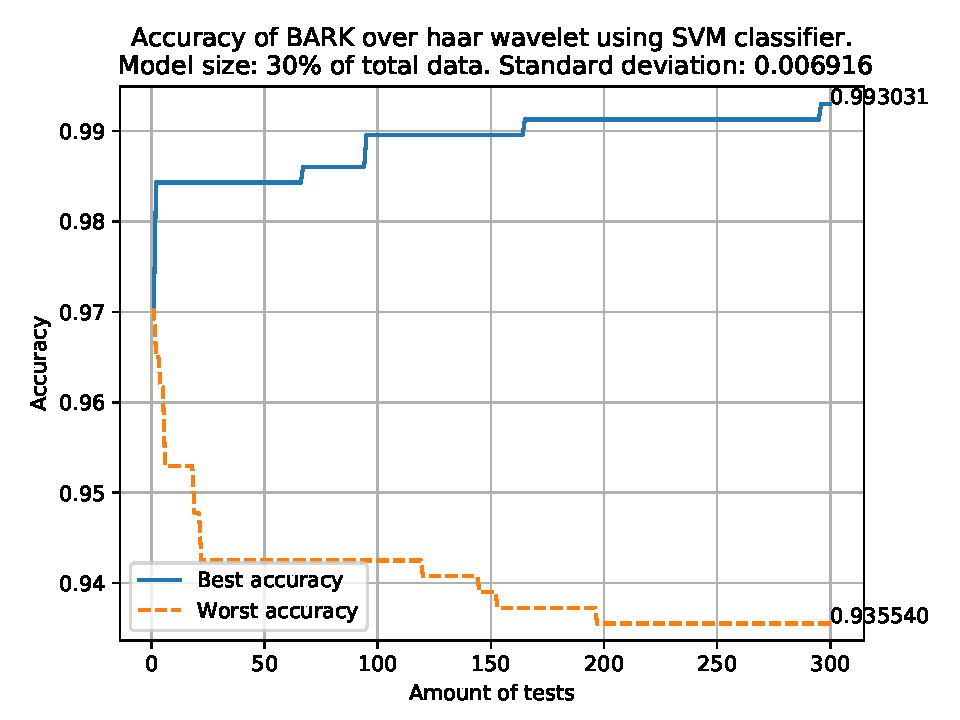
\includegraphics[scale=.8]{images/results/confusionMatrices/classifier_SVM_30.pdf}
		\caption{Accuracy \textit{x} number of tests - SVM with $M=30\%$}
		\label{fig:classifiersvm30}
	\end{figure}
	\begin{figure}[H]
		\centering
		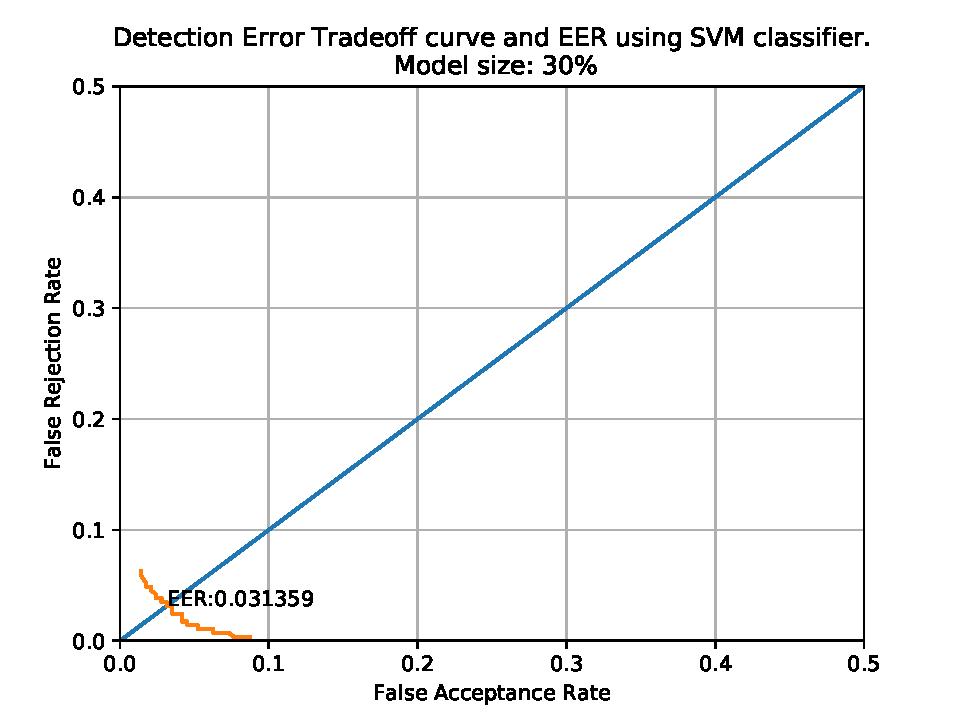
\includegraphics[scale=.8]{images/results/det/DET_for_classifier_SVM_30.pdf}
		\caption{DET curve of SVM results with $M=30\%$}
		\label{fig:detsvm30}
	\end{figure}
	\begin{figure}[H]
		\centering
		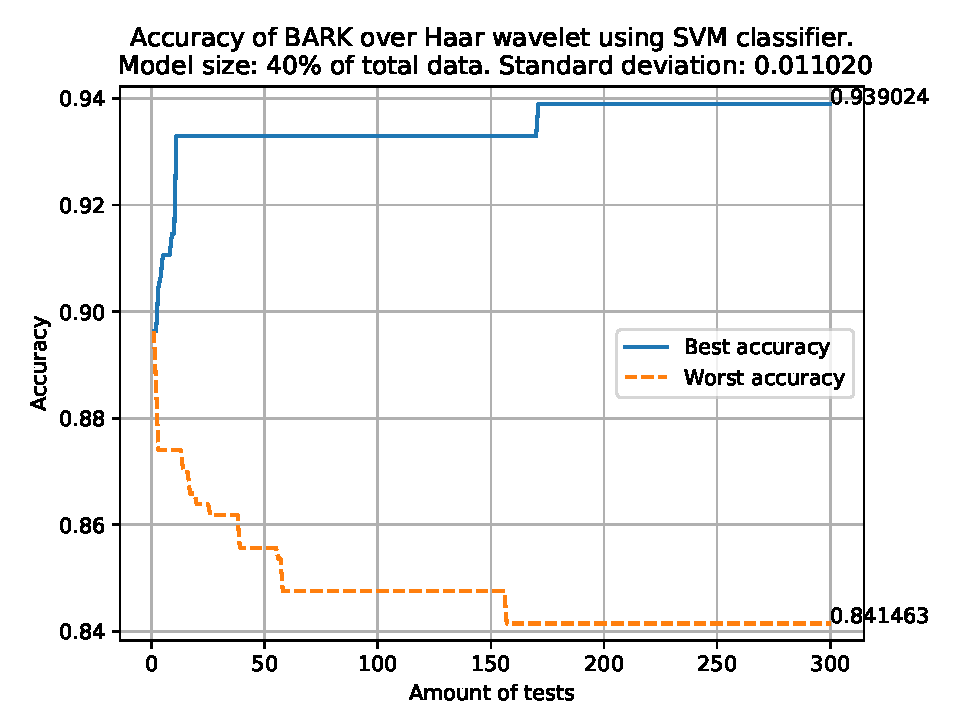
\includegraphics[scale=.8]{images/results/confusionMatrices/classifier_SVM_40.pdf}
		\caption{Accuracy \textit{x} number of tests - SVM with $M=40\%$}
		\label{fig:classifiersvm40}
	\end{figure}
	\begin{figure}[H]
		\centering
		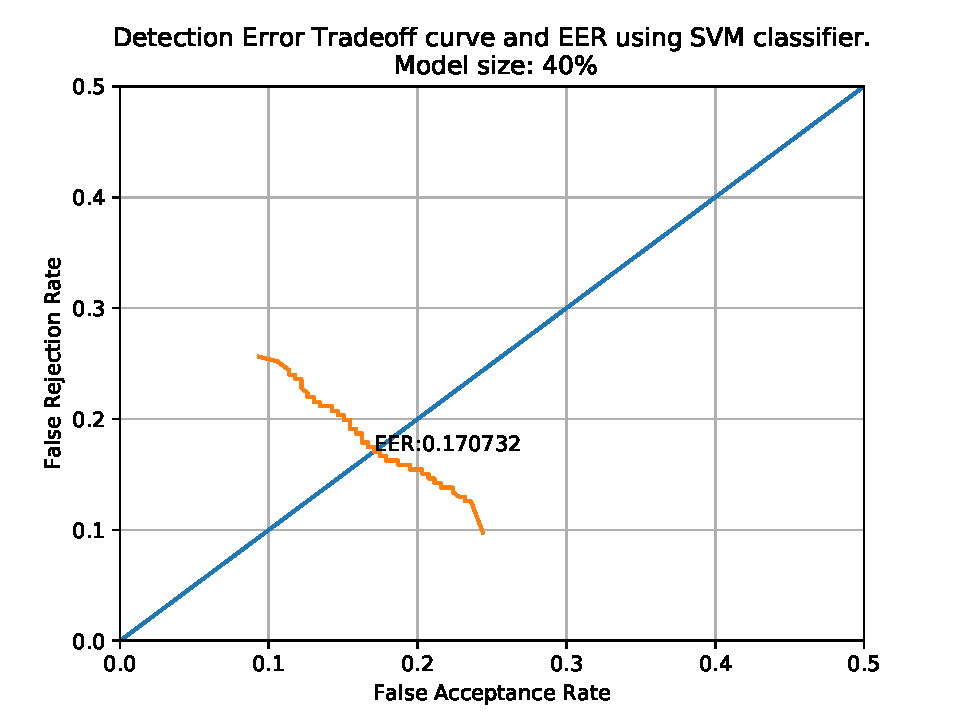
\includegraphics[scale=.8]{images/results/det/DET_for_classifier_SVM_40.pdf}
		\caption{DET curve of SVM results with $M=40\%$}
		\label{fig:detsvm40}
	\end{figure}
	\begin{figure}[H]
		\centering
		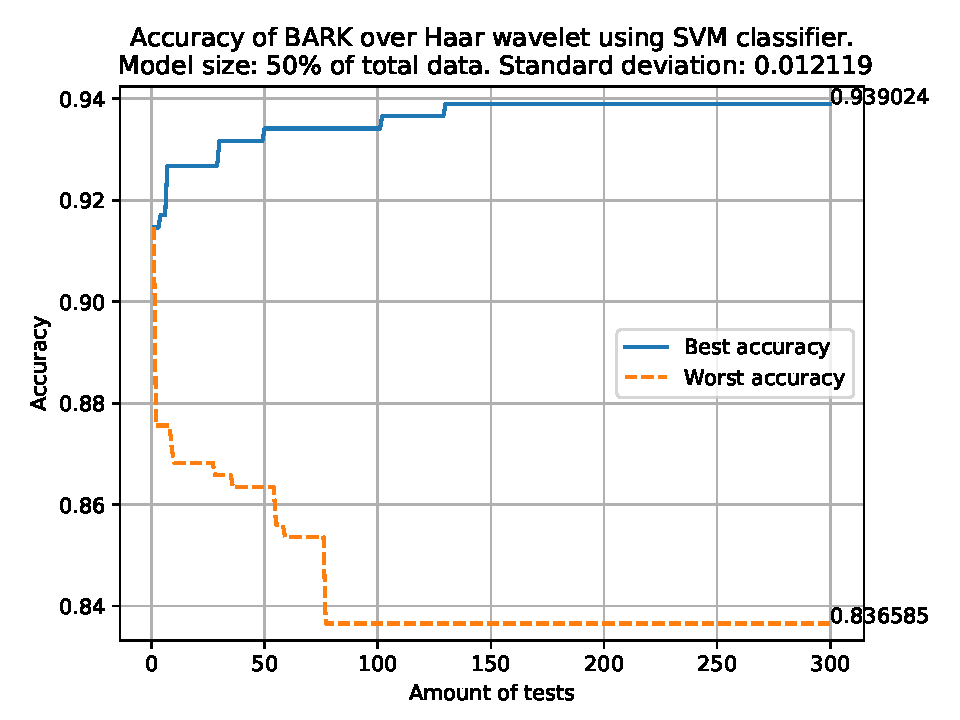
\includegraphics[scale=.8]{images/results/confusionMatrices/classifier_SVM_50.pdf}
		\caption{Accuracy \textit{x} number of tests - SVM with $M=50\%$}
		\label{fig:classifiersvm50}
	\end{figure}
	\begin{figure}[H]
		\centering
		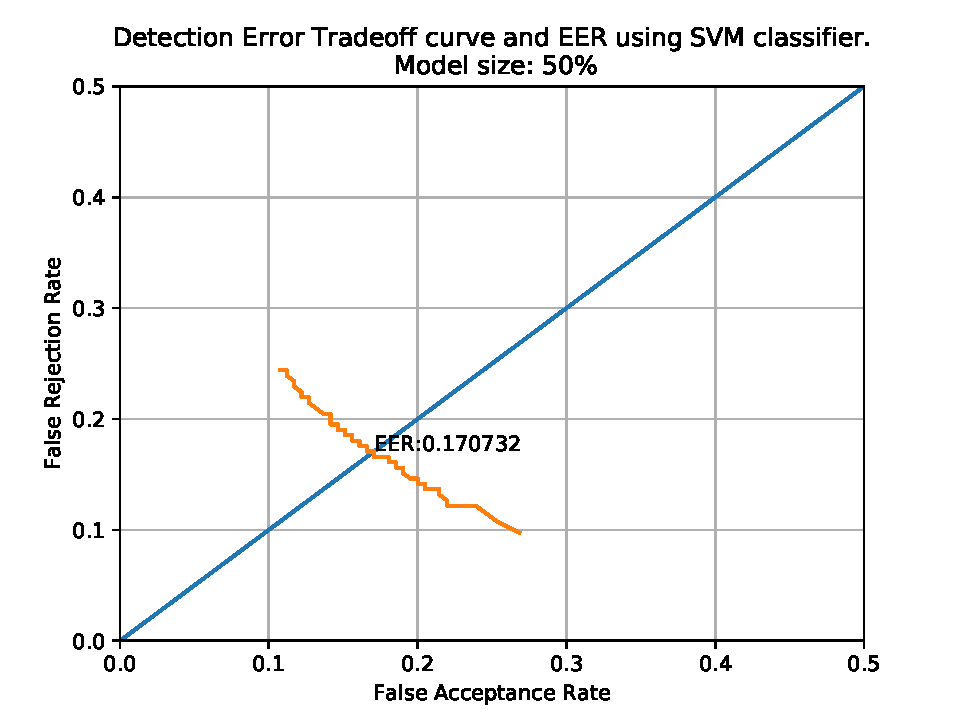
\includegraphics[scale=.8]{images/results/det/DET_for_classifier_SVM_50.pdf}
		\caption{DET curve of SVM results with $M=50\%$}
		\label{fig:detsvm50}
	\end{figure}

	\par In short, the \textbf{best values of accuracy and EER} obtained were \textbf{0.95122 and 0.102439}, respectively, when the SVM classifier was adopted with $M=50\%$, matching the expectations. In such a case, the respective confusion matrix reveals a minimum amount of false-genuine and false-spoofed, consistent with the related works.
	\\
	
	\FloatBarrier
	
	\subsection{Complementary Tests}
		\par Figures \ref{fig:livehaarbark} and \ref{fig:spoofinghaarbark} show, as a complement, scatter plots of the feature vectors values generated by the \textbf{Haar+Bark} pair. Notably, in comparison with Figures \ref{fig:livehaarmel} and \ref{fig:spoofinghaarmel}, the \textbf{spread of values is greater on the Mel scale}. This difference in data distribution also occurs with the pair \textbf{Daubechies 58 + Bark}, as shown in Figures \ref{fig:livedaub58bark} and \ref{fig:spoofingdaub58bark}, in addition to \textbf{Daubechies 58 + Mel}, as per Figures \ref{fig:livedaub58mel} and \ref{fig:spoofingdaub58mel} as well as in \textbf{Coiflets 18 + Bark} and \textbf{Coiflets 18 + Mel} like in Figures \ref{fig:livecoif18bark} and \ref{fig:livecoif18mel}. In this subsection, for the sake of visualization the double derivative of the MEL scale \textbf{was not} taken.
		\\
		\begin{figure}
			\centering
			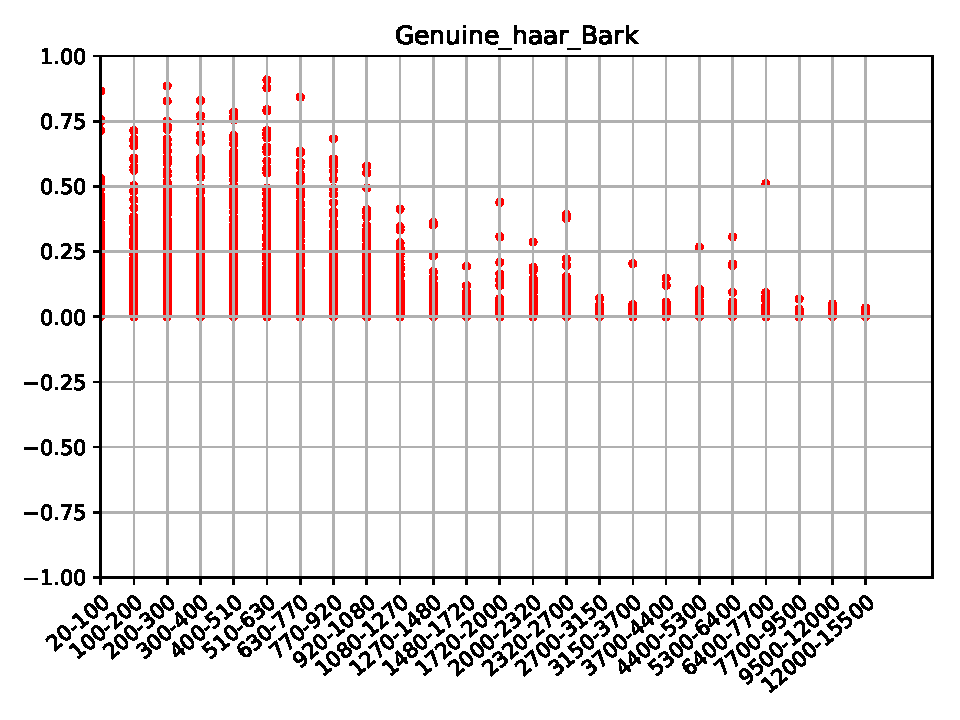
\includegraphics[scale=.7]{images/results/barkVersusMel/Genuine_haar_Bark.pdf}
			\caption{Scatter plot for the \textit{genuine} feature vectors obtained with \textit{Haar + BARK}. Horizontal and vertical axes: frequency bands in Hertz (Hz), and amplitudes, respectively.}
			\label{fig:livehaarbark}
		\end{figure}
		\begin{figure}[H]
			\centering
			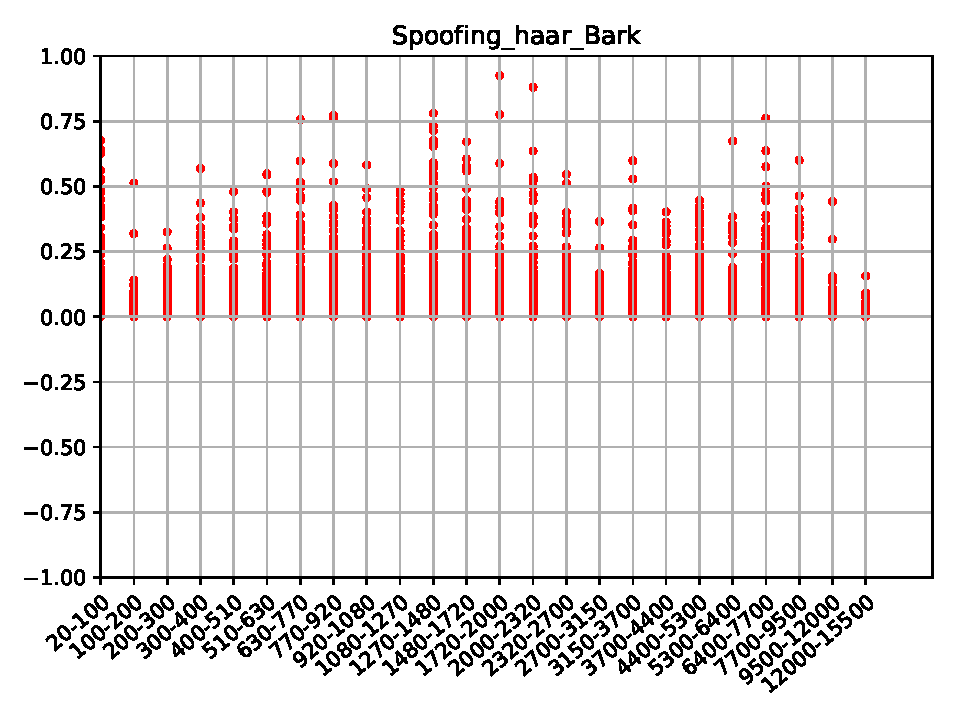
\includegraphics[scale=.7]{images/results/barkVersusMel/Spoofing_haar_Bark.pdf}
			\caption{Scatter plot for the \textit{spoofed} feature vectors obtained with \textit{Haar + BARK}. Horizontal and vertical axes: frequency band, and amplitude, respectively. Horizontal and vertical axes: frequency bands in Hertz (Hz), and amplitudes, respectively.}
			\label{fig:spoofinghaarbark}
		\end{figure}
		\begin{figure}[H]
			\centering
			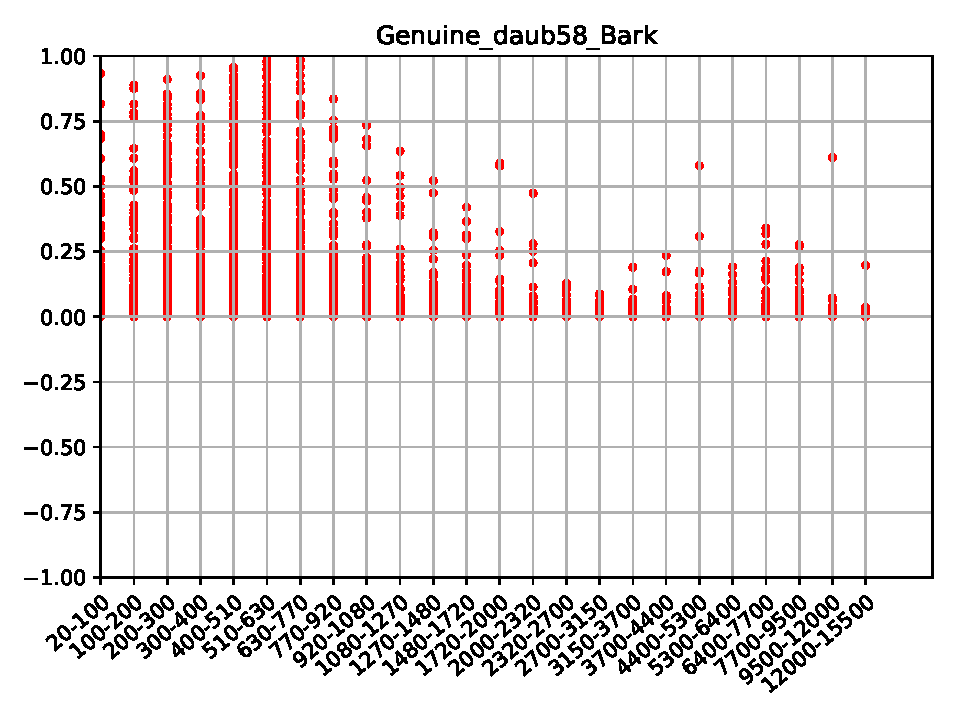
\includegraphics[scale=.7]{images/results/barkVersusMel/Genuine_daub58_Bark.pdf}
			\caption{Scatter plot for \textit{genuine} feature vectors based on the pair \textit{daubechies 58 + BARK}. Horizontal and vertical axes: frequency bands in Hertz (Hz), and amplitudes, respectively.}
			\label{fig:livedaub58bark}
		\end{figure}
		\begin{figure}[H]
			\centering
			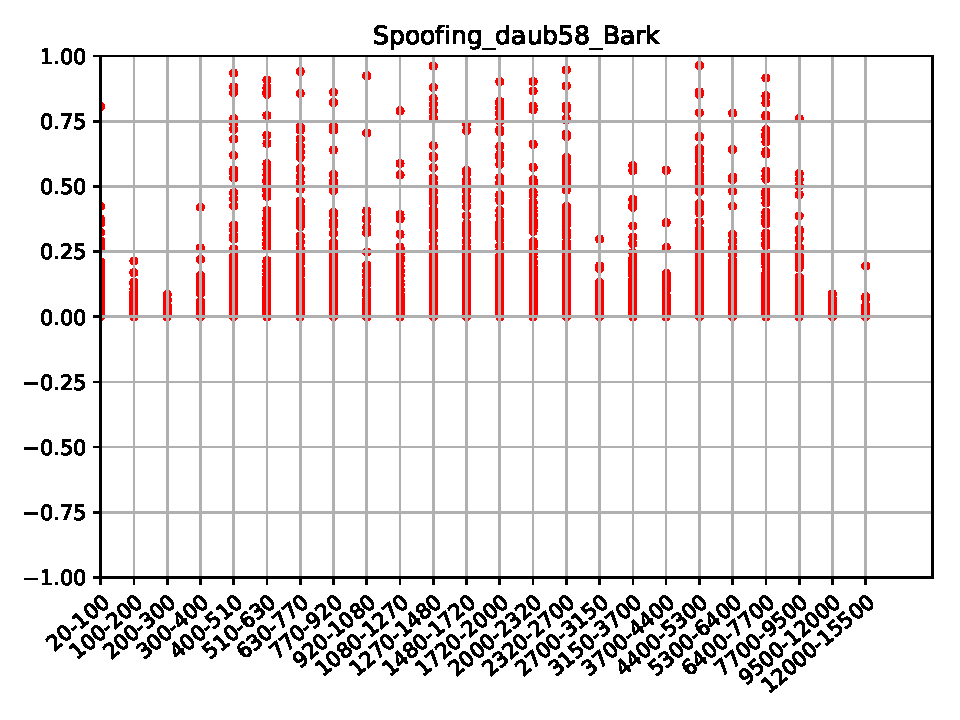
\includegraphics[scale=.7]{images/results/barkVersusMel/Spoofing_daub58_Bark.pdf}
			\caption{Scatter plot for \textit{spoofed} feature vectors based on the pair \textit{daubechies 58 + BARK}. Horizontal and vertical axes: frequency bands in Hertz (Hz), and amplitudes, respectively.}
			\label{fig:spoofingdaub58bark}
		\end{figure}
		\begin{figure}[H]
			\centering
			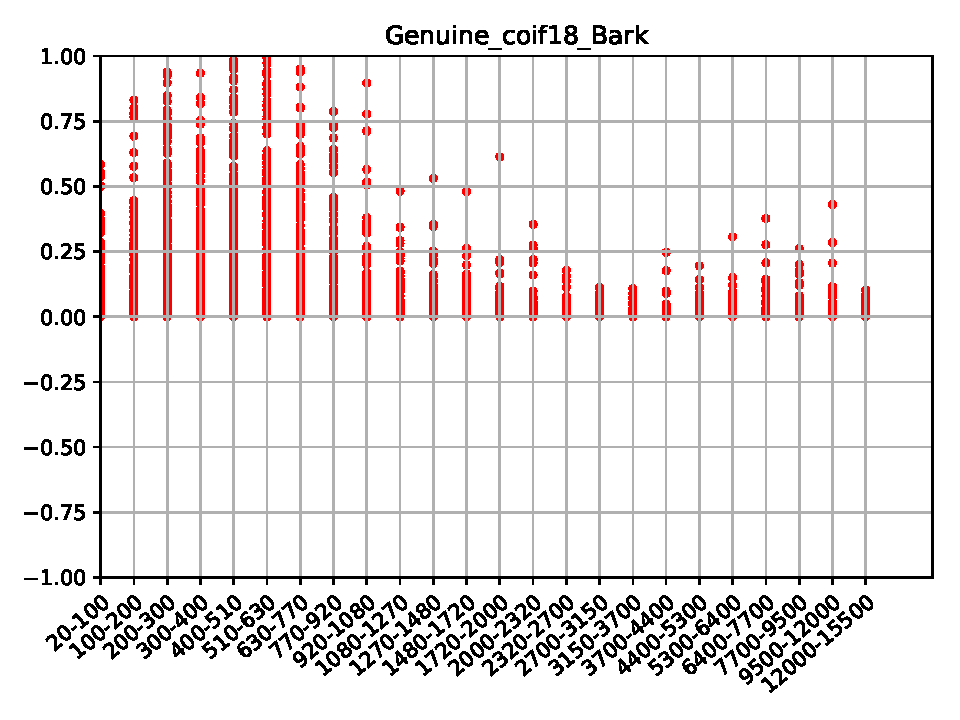
\includegraphics[scale=.7]{images/results/barkVersusMel/Genuine_coif18_Bark.pdf}
			\caption{Scatter plot for \textit{genuine} feature vectors based on the pair \textit{coiflet 18 + BARK}. Horizontal and vertical axes: frequency bands in Hertz (Hz), and amplitudes, respectively.}
			\label{fig:livecoif18bark}
		\end{figure}
		\begin{figure}[H]
			\centering
			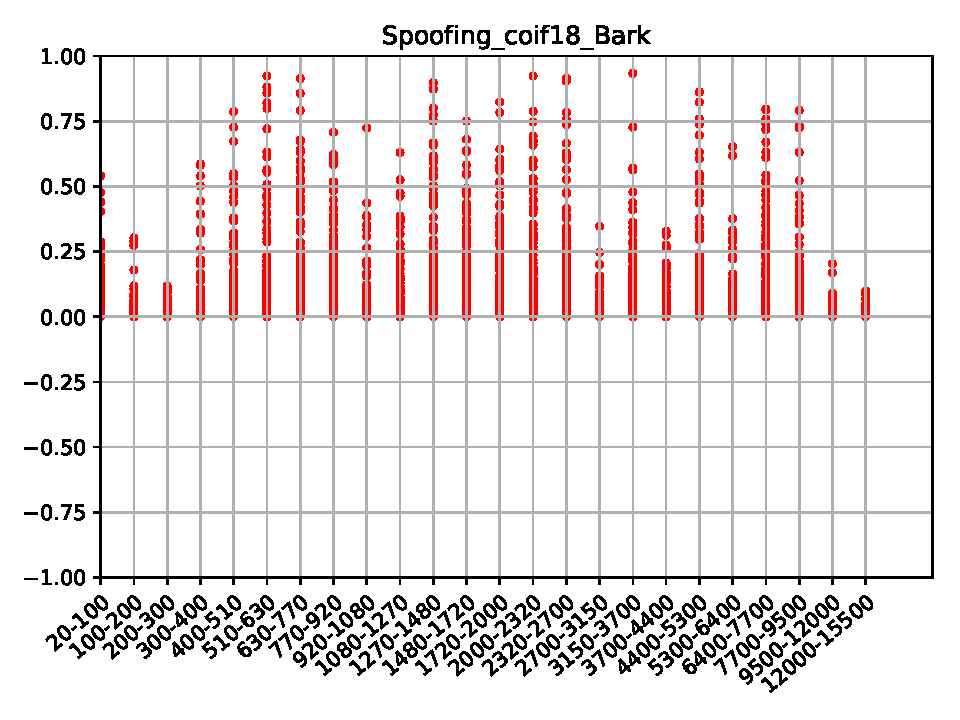
\includegraphics[scale=.7]{images/results/barkVersusMel/Spoofing_coif18_Bark.pdf}
			\caption{Scatter plot for \textit{spoofed} feature vectors based on the pair \textit{coiflet 18 + BARK}. Horizontal and vertical axes: frequency bands in Hertz (Hz), and amplitudes, respectively.}
			\label{fig:spoofingcoif18bark}
		\end{figure}
		\begin{figure}[H]
			\centering
			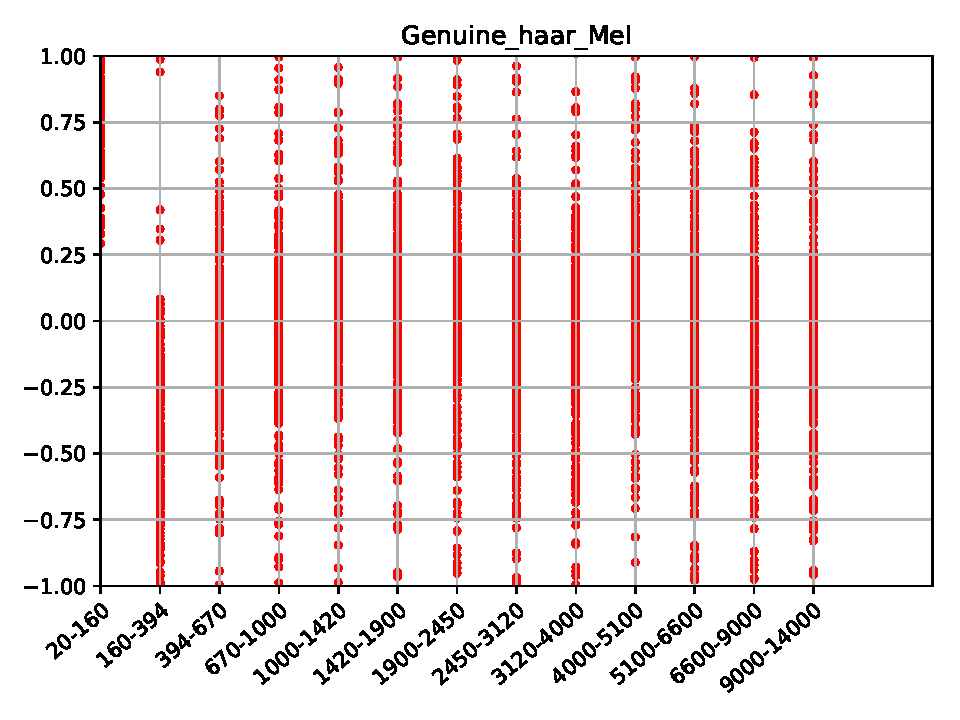
\includegraphics[scale=.7]{images/results/barkVersusMel/Genuine_haar_Mel.pdf}
			\caption{Scatter plot for \textit{genuine} feature vectors based on the pair \textit{Haar + MEL}. Horizontal and vertical axes: frequency bands in Hertz (Hz), and amplitudes, respectively.}
			\label{fig:livehaarmel}
		\end{figure}
		\begin{figure}[H]
			\centering
			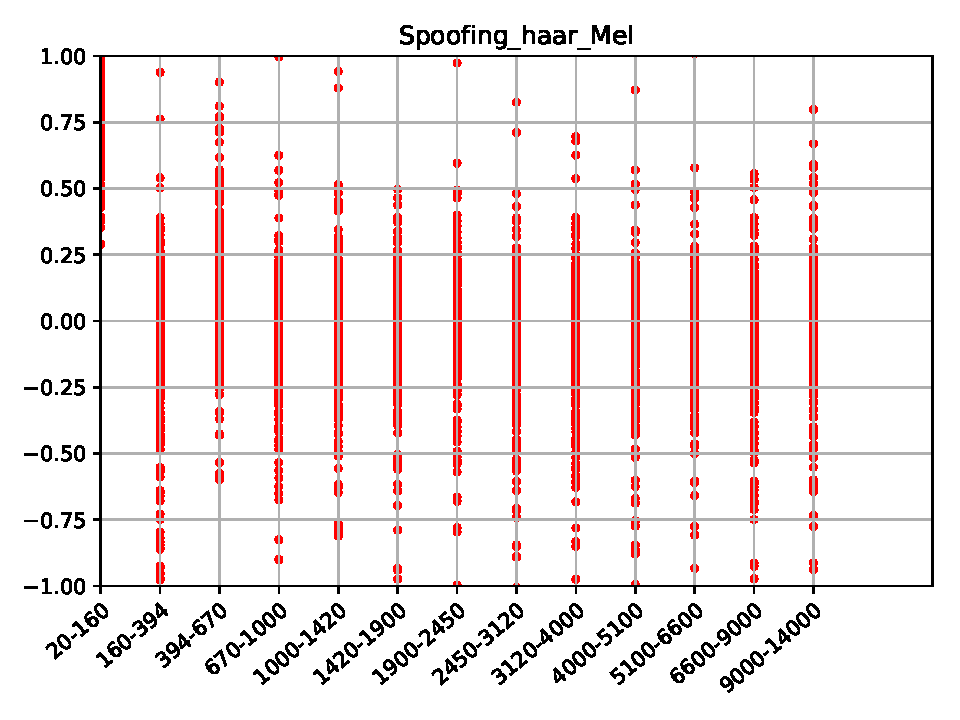
\includegraphics[scale=.7]{images/results/barkVersusMel/Spoofing_haar_Mel.pdf}
			\caption{Scatter plot for \textit{spoofed} feature vectors based on the pair \textit{Haar + MEL}. Horizontal and vertical axes: frequency bands in Hertz (Hz), and amplitudes, respectively.}
			\label{fig:spoofinghaarmel}
		\end{figure}
		\begin{figure}[H]
			\centering
			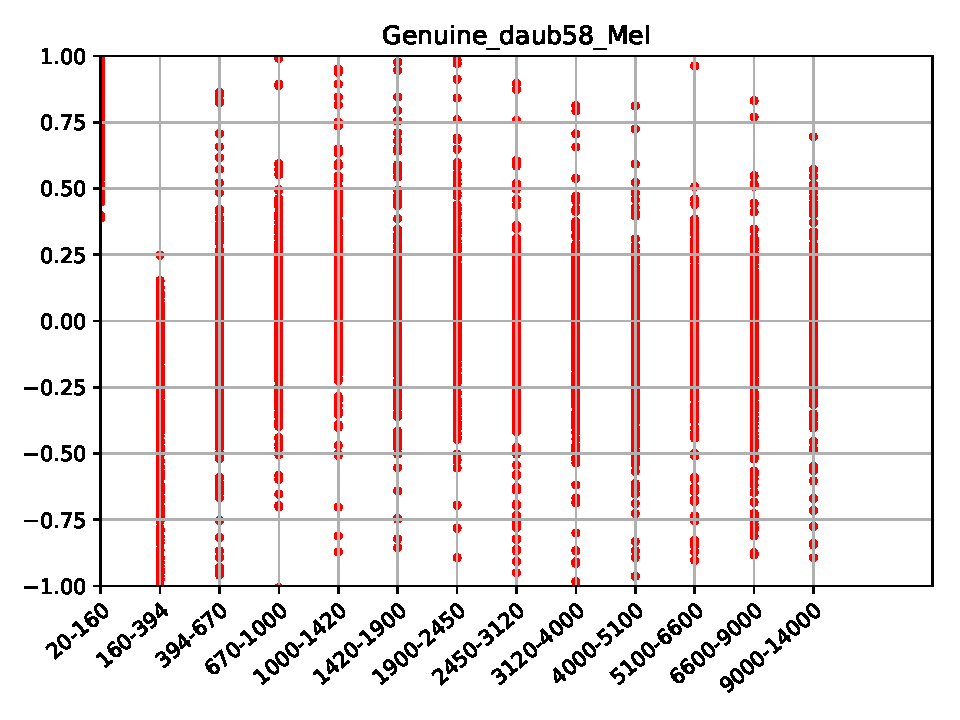
\includegraphics[scale=.7]{images/results/barkVersusMel/Genuine_daub58_Mel.pdf}
			\caption{Scatter plot for \textit{genuine} feature vectors  based on the pair \textit{daubechies 58 + MEL}. Horizontal and vertical axes: frequency bands in Hertz (Hz), and amplitudes, respectively.}
			\label{fig:livedaub58mel}
		\end{figure}
		\begin{figure}[H]
			\centering
			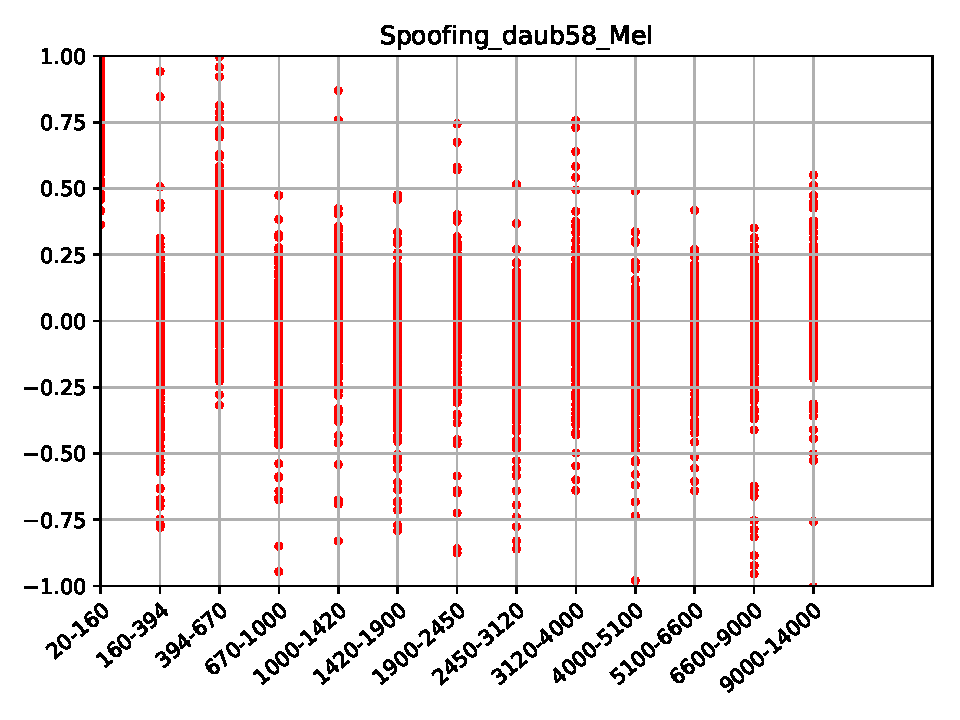
\includegraphics[scale=.7]{images/results/barkVersusMel/Spoofing_daub58_Mel.pdf}
			\caption{Scatter plot for \textit{spoofed} feature vectors  based on the pair \textit{daubechies 58 + MEL}. Horizontal and vertical axes: frequency bands in Hertz (Hz), and amplitudes, respectively.}
			\label{fig:spoofingdaub58mel}
		\end{figure}	
		\begin{figure}[H]
			\centering
			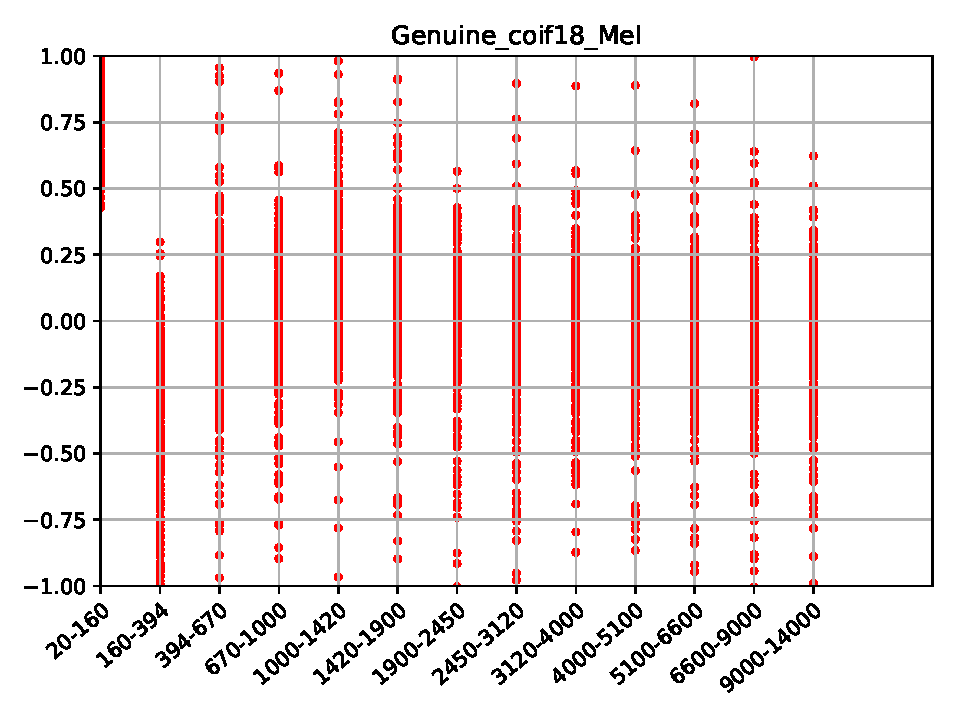
\includegraphics[scale=.7]{images/results/barkVersusMel/Genuine_coif18_Mel.pdf}
			\caption{Scatter plot for \textit{genuine} feature vectors  based on the pair \textit{coiflet 18 + MEL}. Horizontal and vertical axes: frequency bands in Hertz (Hz), and amplitudes, respectively.}
			\label{fig:livecoif18mel}
		\end{figure}
		\begin{figure}[H]
			\centering
			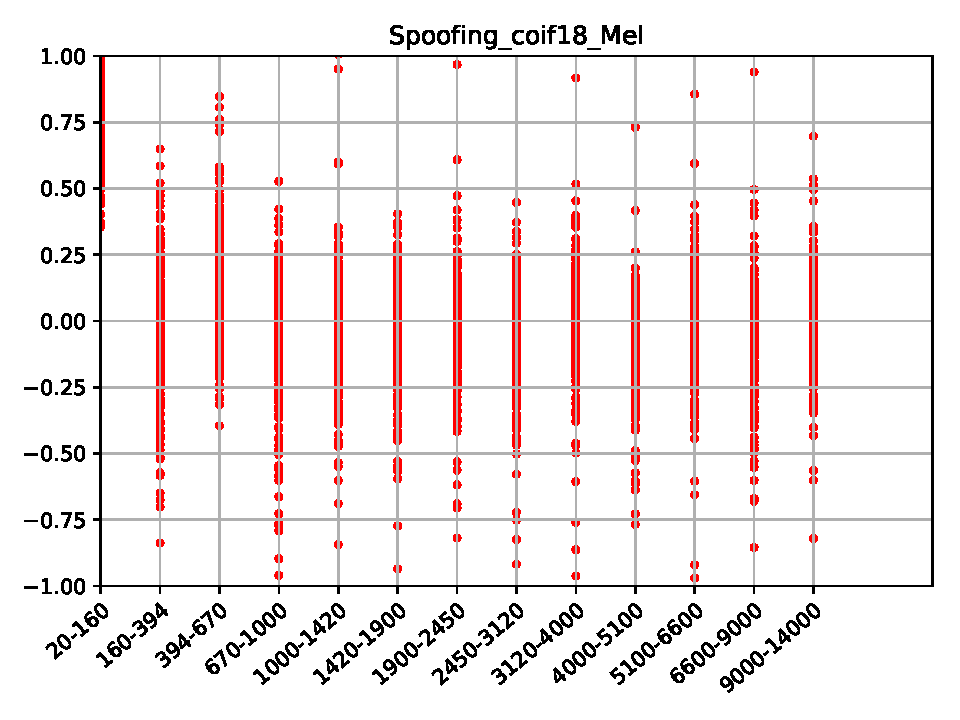
\includegraphics[scale=.7]{images/results/barkVersusMel/Spoofing_coif18_Mel.pdf}
			\caption{Scatter plot for \textit{spoofed} feature vectors  based on the pair \textit{coiflet 18 + MEL}. Horizontal and vertical axes: frequency bands in Hertz (Hz), and amplitudes, respectively.}
			\label{fig:spoofingcoif18mel}
		\end{figure}